\chapter{Methodology}
\label{ch:methodology}

This chapter presents the methodology developed for extracting vectorized lane markings from raw mobile LiDAR point clouds. Section~\ref{sec:inputoutput} describes the input data and the expected output format. Section~\ref{sec:pipeline_overview} provides a high-level overview of the processing pipeline. Sections~\ref{sec:car_trace}--\ref{sec:line_fitting} detail the three major stages of the pipeline: vehicle trajectory reconstruction, point cloud processing, and line fitting.

\section{Input Data and Expected Output}
\label{sec:inputoutput}

The input data received from TomTom consists of approximately $10\,\mathrm{km}$ of globally georeferenced LiDAR data in the EPSG:3857 (Web Mercator) coordinate system. No vehicle trajectory was provided with the dataset. The data is spatially partitioned into H3 hexagonal cells at resolution~7. The two relevant cells are \texttt{871e1d8b1ffffff} and \texttt{871e1d886ffffff} (see Figure~\ref{fig:h3cells}). From the available point attributes, the coordinates $(x,y,z)$, \texttt{gps\_timestamp}, and \texttt{intensity} were retained for processing. The intensity value corresponds to the reflectivity of the observed surface.

\begin{figure}[htbp]
  \centering
  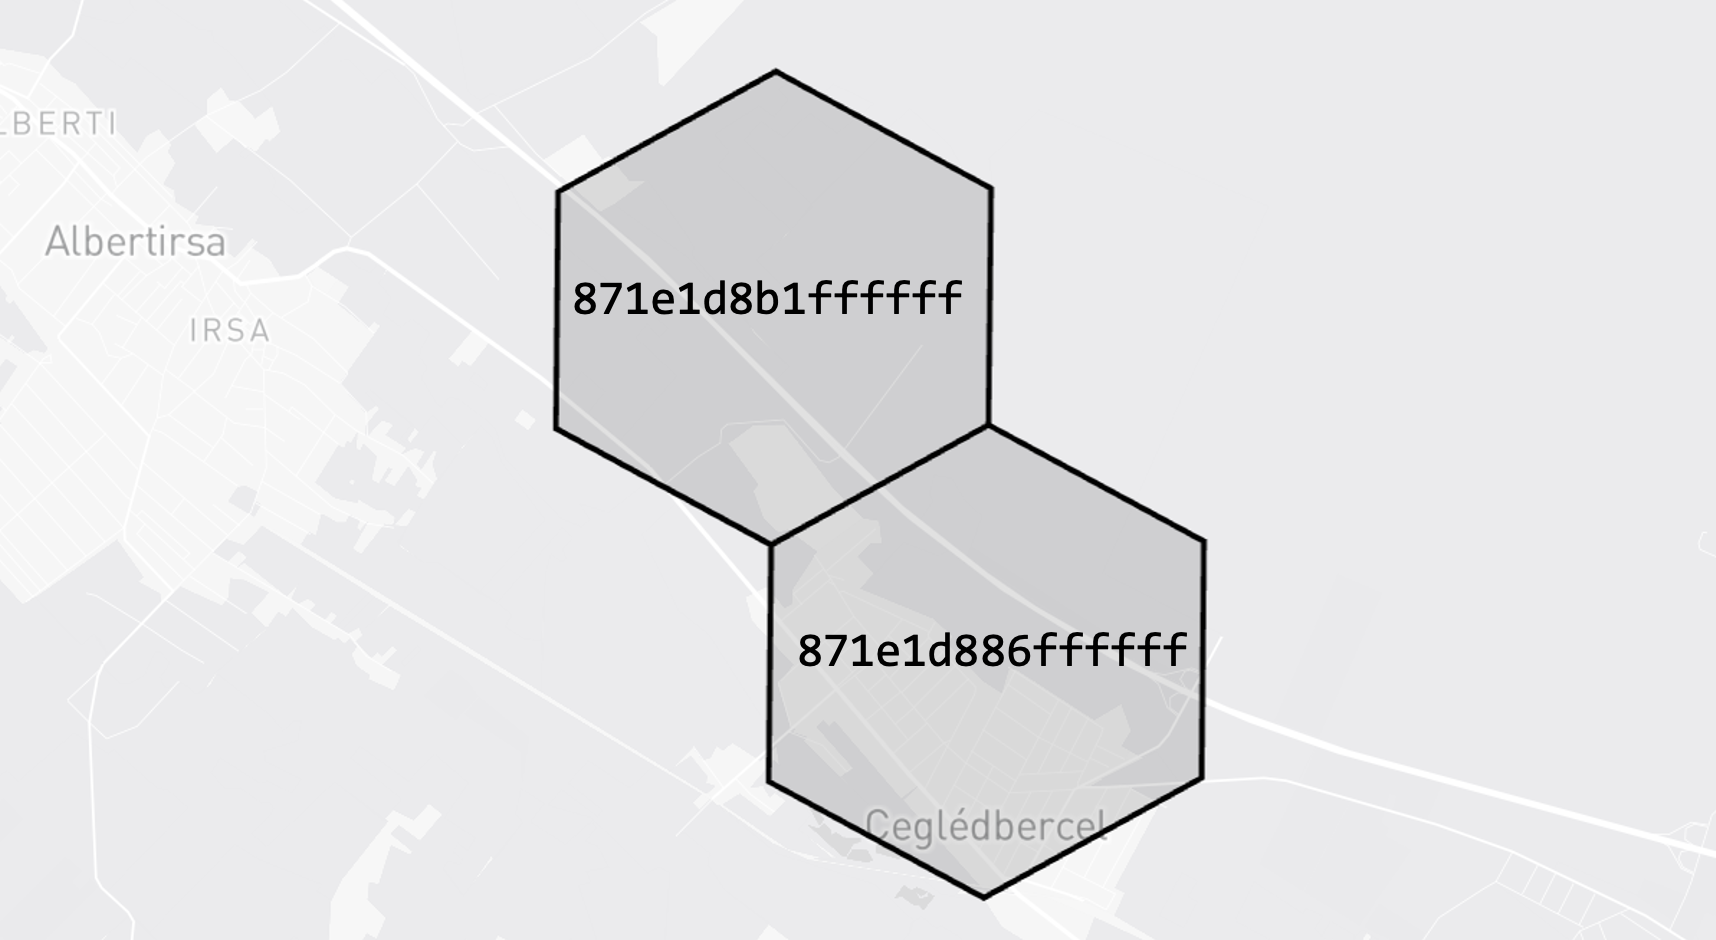
\includegraphics[width=0.7\textwidth]{images/inputdata/h3cells}
  \caption{The two H3 cells covering the captured highway section.}
  \label{fig:h3cells}
\end{figure}

Each cell contains approximately 100 million points. The intensity values range from~0 to~255, where~255 corresponds to the highest reflectivity. In cell \texttt{871e1d886ffffff}, the difference between the minimum and maximum GPS timestamp values is approximately $235\,\mathrm{s}$, indicating that the Mobile Mapping (MoMa) session traversed the highway section (in both directions) in slightly more than three minutes (see Figure~\ref{fig:cegl2gpstime}).

\begin{figure}[htbp]
  \centering
  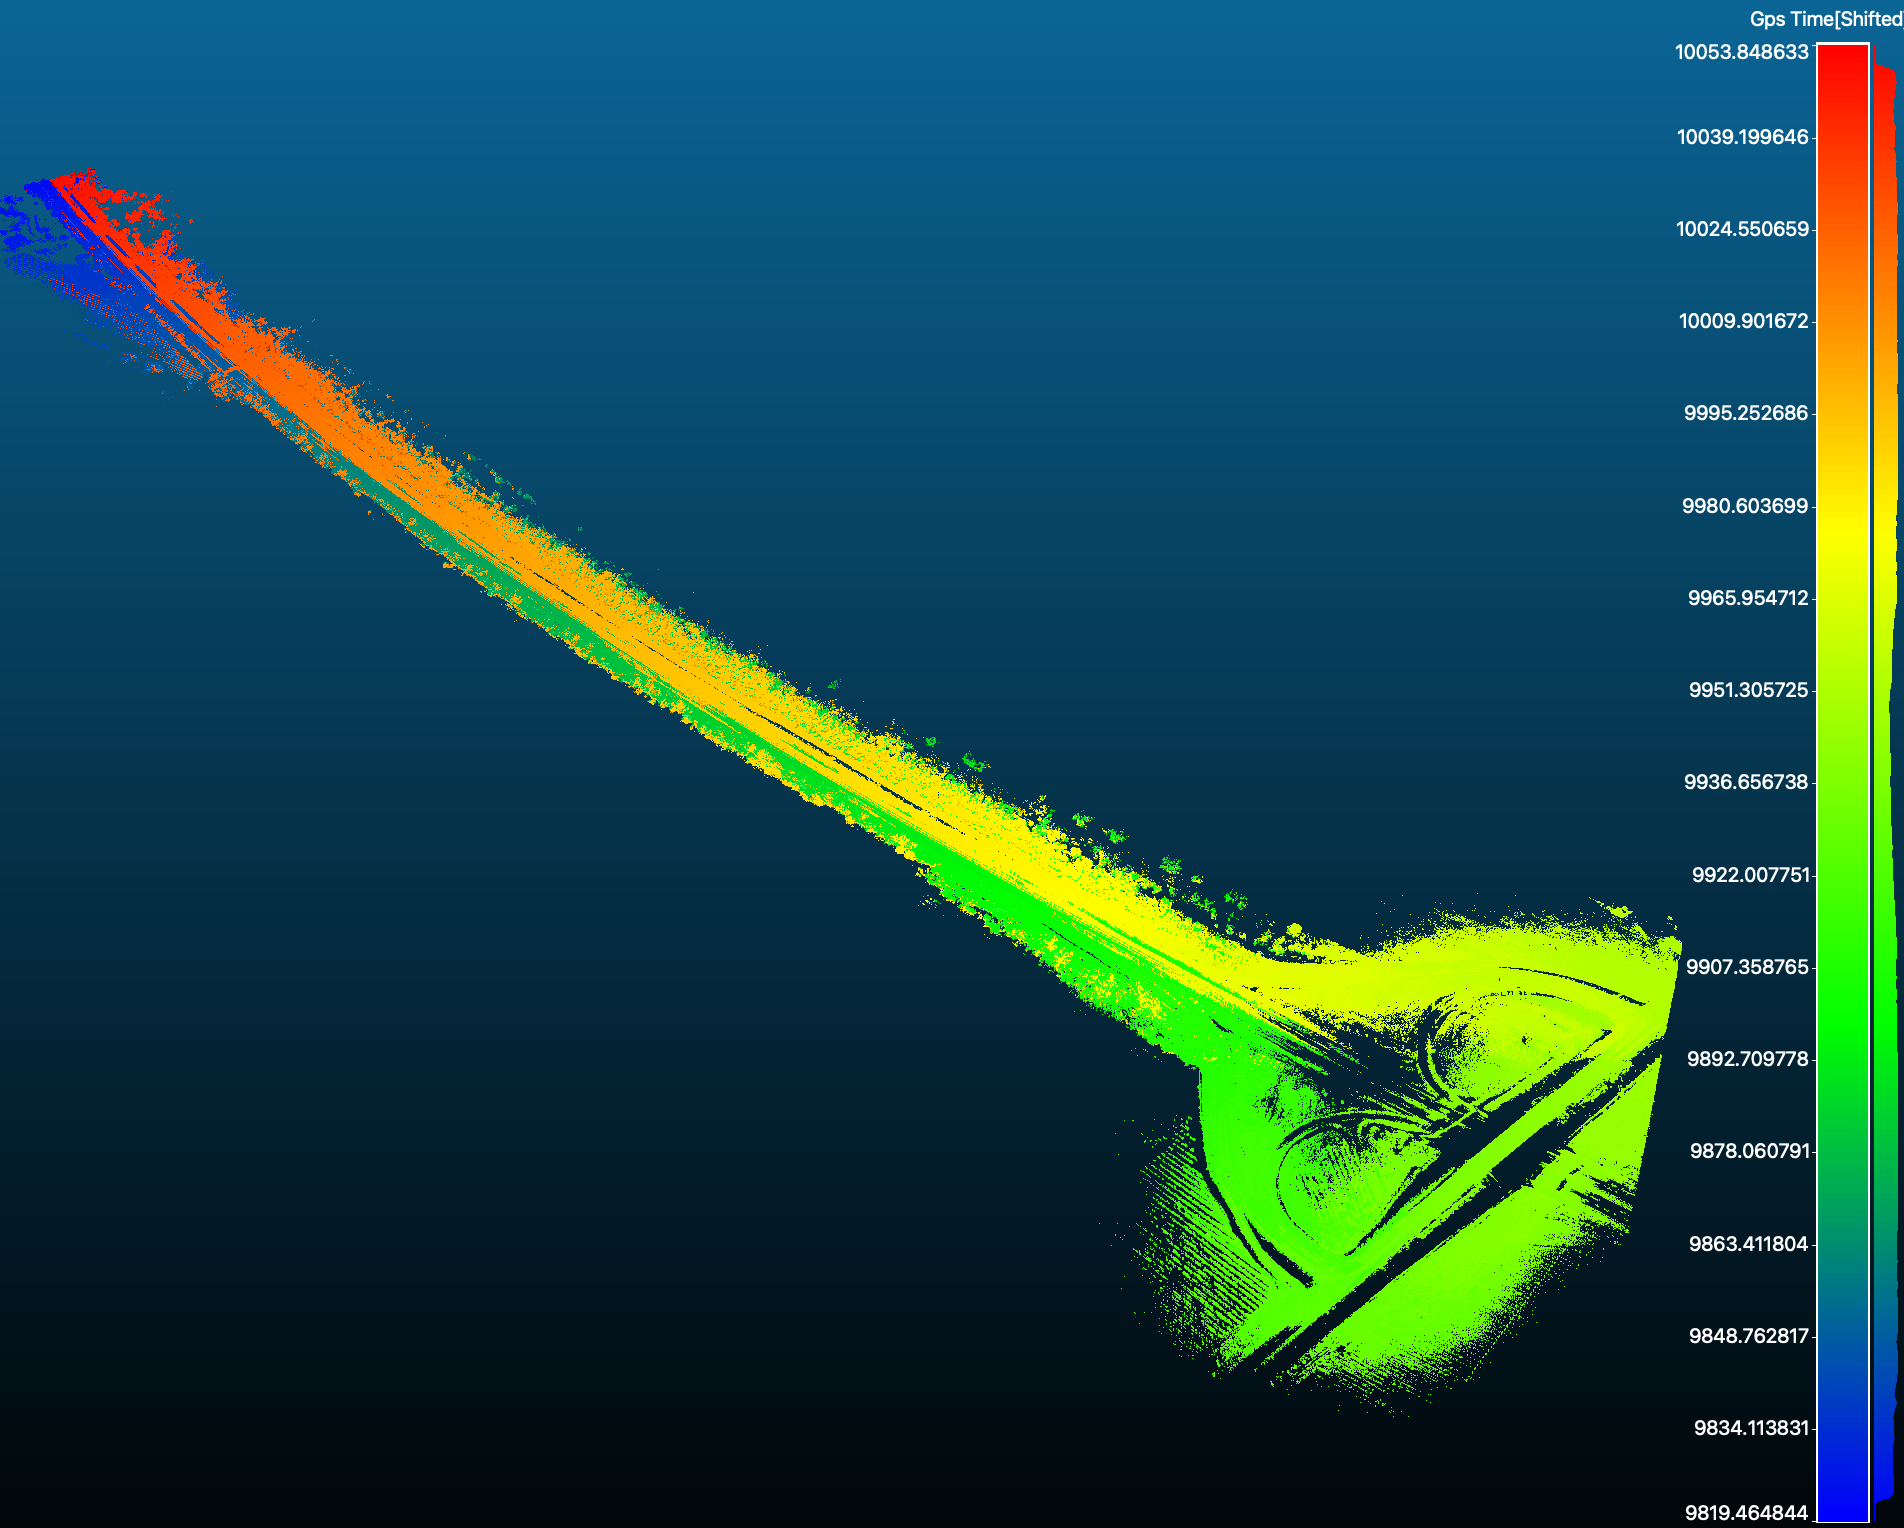
\includegraphics[width=0.7\textwidth]{images/inputdata/cegl2bytime}
  \caption{LiDAR data of cell \texttt{871e1d886ffffff} colored by GPS timestamp.}
  \label{fig:cegl2gpstime}
\end{figure}

\FloatBarrier
\subsection{Sensor Characteristics}
\label{sec:sensor}

The point cloud was captured using a Velodyne HDL-32E LiDAR sensor featuring 32 vertically stacked laser channels. During each firing sequence, the sensor emits one pulse per laser beam, yielding 32 distance measurements. A complete 32-laser firing sequence is generated every $46\,\mu\mathrm{s}$, corresponding to an effective firing frequency of approximately $21.7\,\mathrm{kHz}$.

Every 24 consecutive firing sequences are grouped into a single UDP packet, and all points within a packet share the same GPS timestamp. Consequently, each packet contains
\begin{equation}
  N_{\text{packet}} = 24 \times 32 = 768 \text{ measured points.}
  \label{eq:packet_size}
\end{equation}
\noindent In practice, fewer points are recorded because some emitted laser beams do not produce a valid return signal. Based on these values, the packet rate is approximately $900$~packets per second.

The laser channels rotate around a vertical axis at $20\,\mathrm{Hz}$, meaning that one full revolution takes $0.05\,\mathrm{s}$. Consequently, approximately 45~packets are generated during a single revolution, and each packet corresponds to roughly an $8^{\circ}$ azimuth sector of the environment, as illustrated in Figure~\ref{fig:lidarpackets}.

\begin{figure}[htbp]
  \centering
  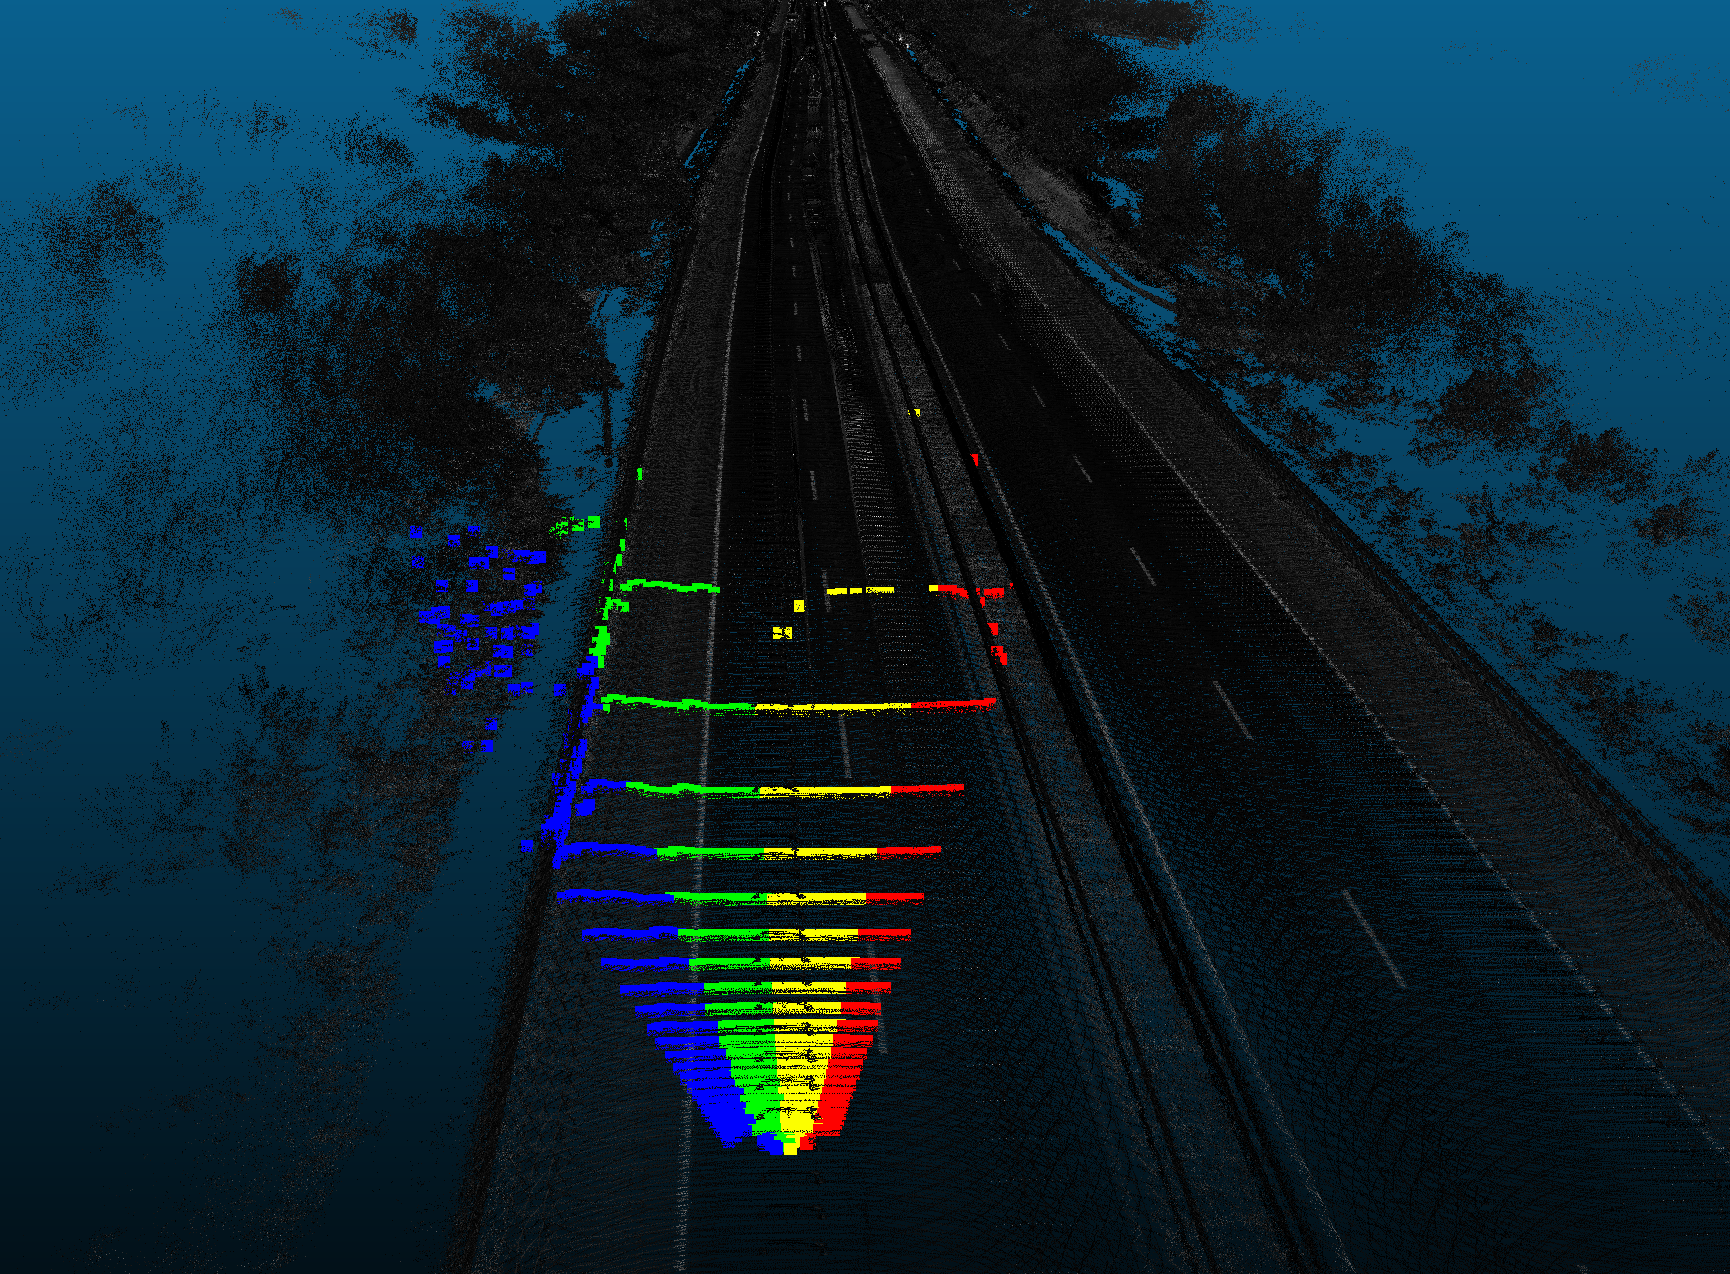
\includegraphics[width=0.7\textwidth]{images/inputdata/lidarpackets}
  \caption{A portion of the point cloud colored by intensity, with individual packets highlighted by their GPS timestamps.}
  \label{fig:lidarpackets}
\end{figure}

\FloatBarrier
\subsection{Data Structure}
\label{sec:datastructure}

By their nature, point clouds are unorganized data that require structured processing before they can be used for autonomous driving applications or, in this case, ground truth generation for road cross-sections. Table~\ref{tab:pointcloud_sample} shows a representative sample of the input data.

\begin{table}[htbp]
  \centering
  \caption{Sample records from the input point cloud.}
  \label{tab:pointcloud_sample}
  \begin{tabular}{rrrrr}
    \hline
    $x$ & $y$ & $z$ & Intensity & Timestamp \\
    \hline
    2192262.82 & 5978199.32 & 159.39 & 3  & 29922.606117 \\
    2192259.85 & 5978197.97 & 159.34 & 6  & 29922.606117 \\
    2192258.76 & 5978197.48 & 159.32 & 6  & 29922.606117 \\
    2192257.82 & 5978197.05 & 159.31 & 3  & 29922.606117 \\
    2192257.06 & 5978196.70 & 159.29 & 0  & 29922.606117 \\
    2192256.34 & 5978196.38 & 159.28 & 1  & 29922.606117 \\
    2192255.78 & 5978196.11 & 159.26 & 2  & 29922.606117 \\
    2192255.20 & 5978195.86 & 159.26 & 41 & 29922.606117 \\
    \hline
  \end{tabular}
\end{table}

\FloatBarrier
\subsection{Expected Output}
\label{sec:expected_output}

The expected output is a vectorized representation of the lane marking geometries along the recorded highway section. This representation is intended for generating ground truth cross-sections. Each geometry must be labeled according to its type: \emph{solid} or \emph{dashed}. The pipeline produces a GeoPackage file containing multiple LineString geometries, each annotated with a \texttt{type} attribute set to either \texttt{solid} or \texttt{dashed}.

%------------------------------------------------------------------
\section{Pipeline Overview}
\label{sec:pipeline_overview}

The pipeline consists of multiple interdependent processing stages organized into three major phases (see Figure~\ref{fig:process}):

\begin{enumerate}
  \item \textbf{Vehicle trajectory reconstruction} (Section~\ref{sec:car_trace}):
  \begin{enumerate}
    \item Reconstruct the vehicle trajectory from LiDAR timestamps, providing an initial estimate of the lane positions.
  \end{enumerate}

  \item \textbf{Point cloud processing} (Section~\ref{sec:pointcloud_processing}):
  \begin{enumerate}
    \item Bin the point cloud along the vehicle trace and process it in overlapping windows.
    \item Remove distant points using trace-based clipping.
    \item Segment ground and non-ground points using RANSAC-based plane detection~\cite{RANSAC}.
    \item Detect the road surface using region-growing methods seeded from the trace.
    \item Segment road markings using intensity thresholding (Kapur maximum-entropy method~\cite{KAPUR1985273} or percentile-based thresholding).
  \end{enumerate}

  \item \textbf{Line fitting on road markings} (Section~\ref{sec:line_fitting}):
  \begin{enumerate}
    \item Cluster and track lane marking points across overlapping windows.
    \item Fit and refine vectorized lane curves using constrained quadratic RANSAC and moving least squares.
    \item Label lane types (solid or dashed) based on point continuity.
  \end{enumerate}
\end{enumerate}

\noindent Finally, the detected lanes are exported as georeferenced vector representations.

\begin{figure}[htbp]
  \centering
  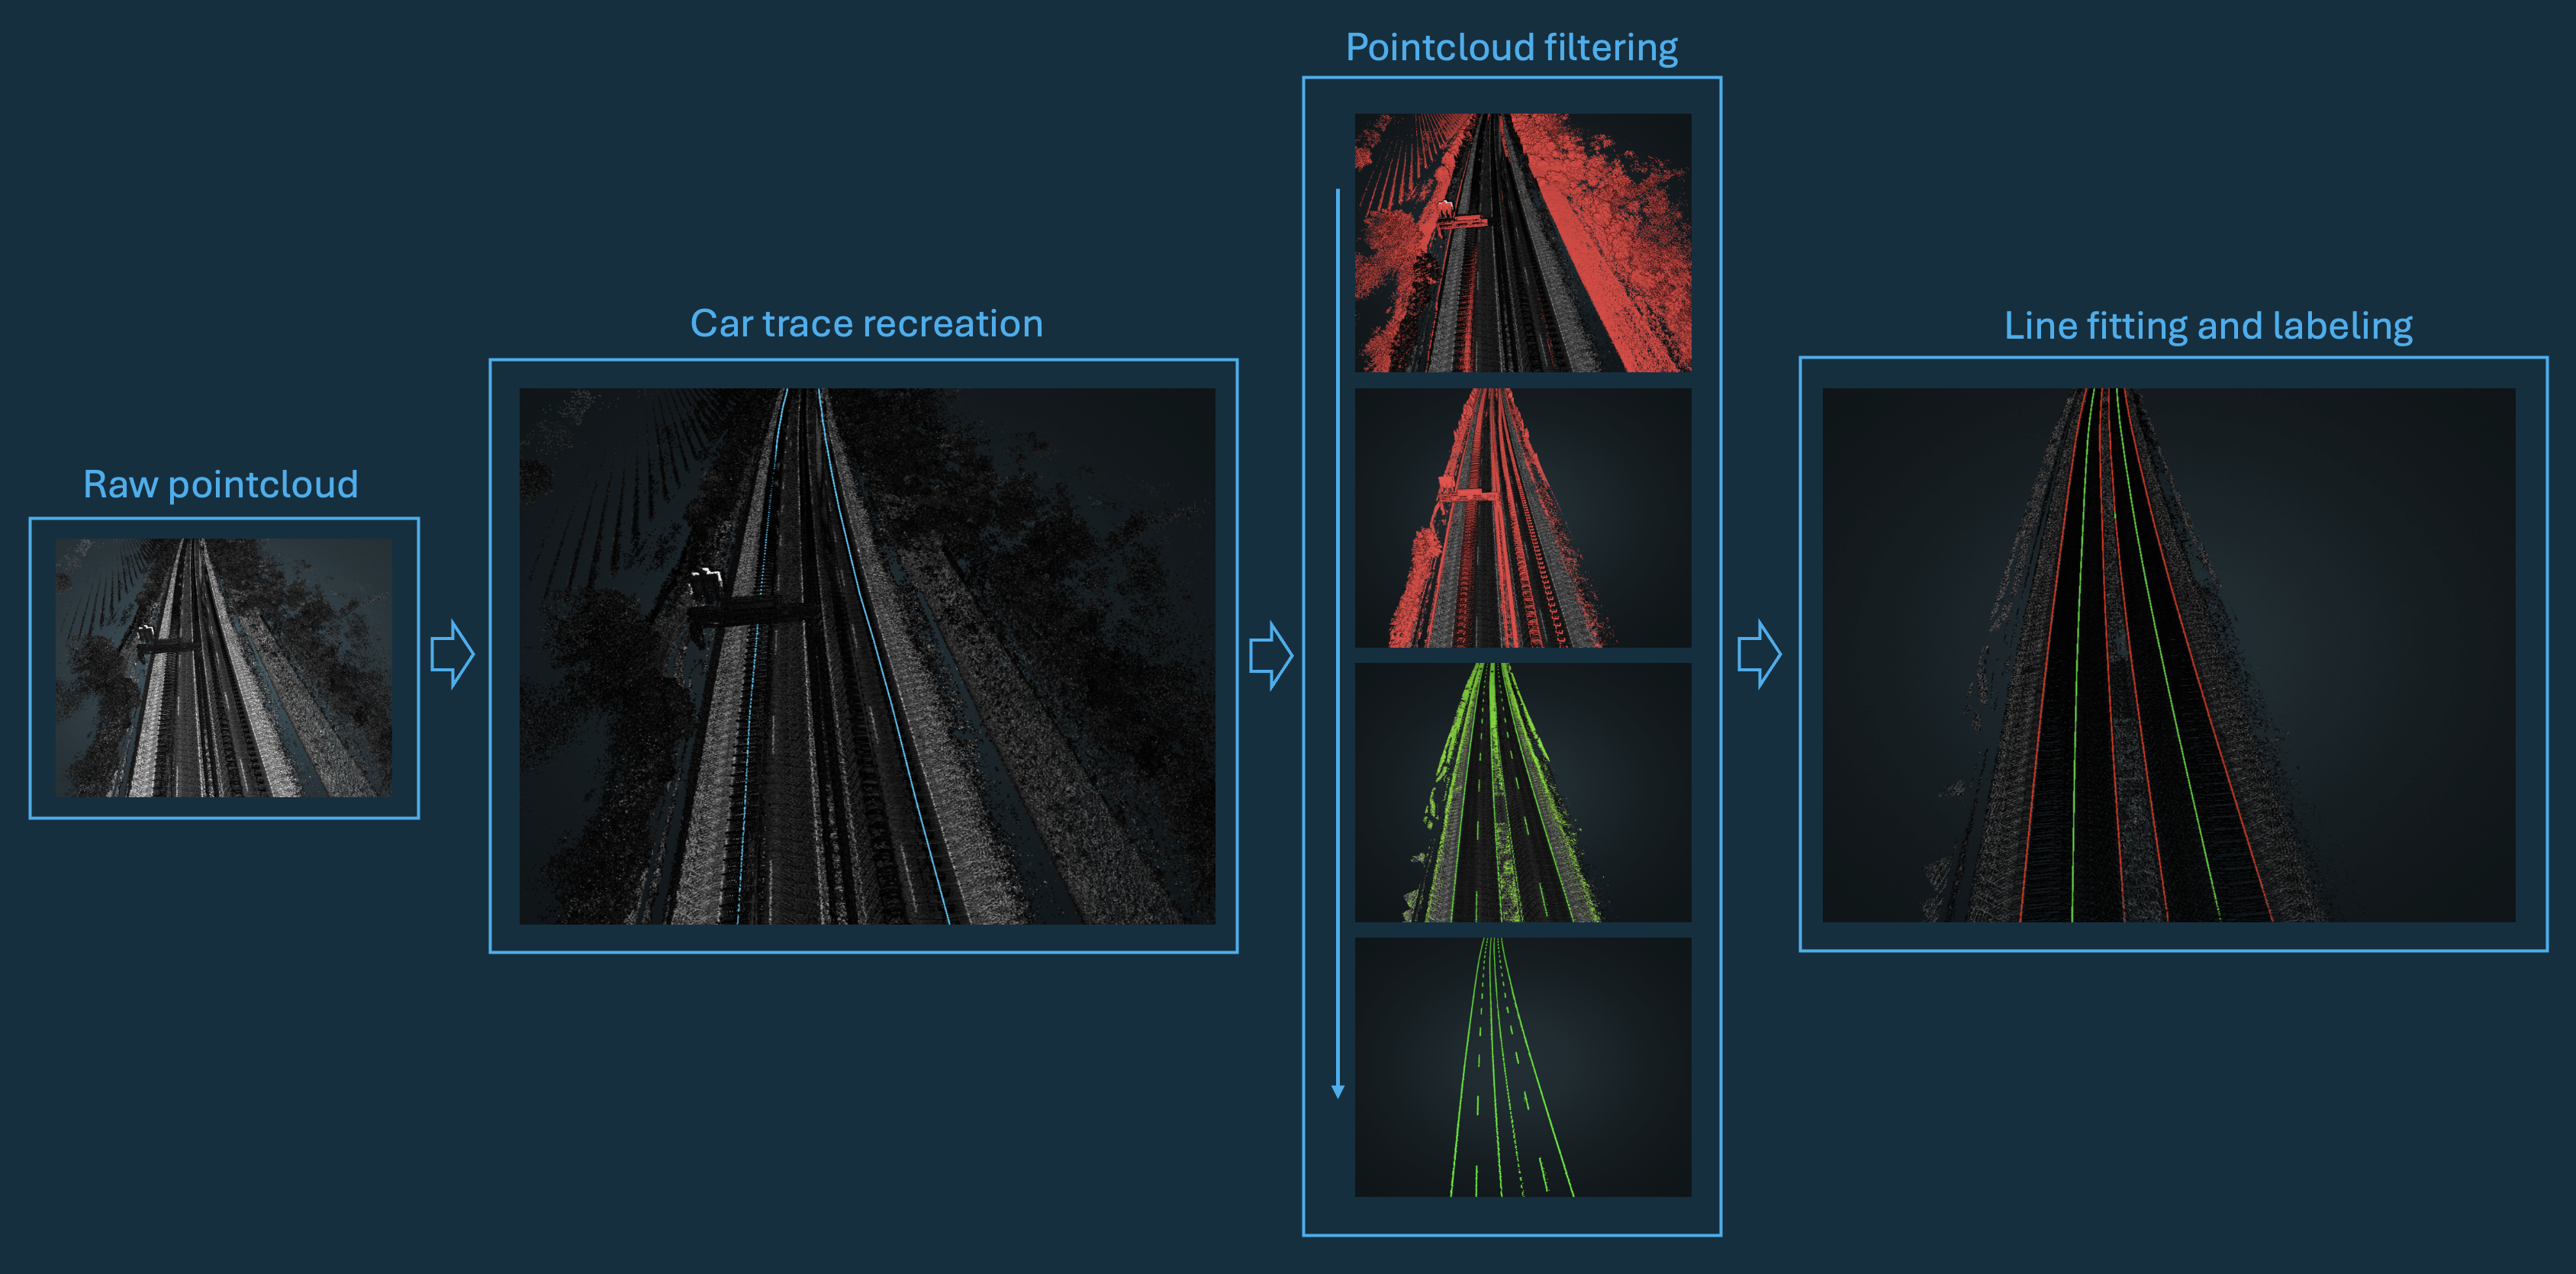
\includegraphics[width=0.9\textwidth]{images/process}
  \caption{High-level overview of the lane detection pipeline, showing the three major phases: trajectory reconstruction, point cloud processing, and line fitting.}
  \label{fig:process}
\end{figure}

%------------------------------------------------------------------
\section{Vehicle Trajectory Reconstruction}
\label{sec:car_trace}

Knowledge of the mapping vehicle's trajectory is essential for the pipeline. Given the trajectory, an initial estimate of the lane positions can be derived, since the vehicle is assumed to have traveled within a lane throughout the recording session. However, since no trajectory data was provided with the dataset, it must be recovered from the properties of the point cloud itself.

The following assumptions are made:
\begin{itemize}
  \item The MoMa vehicle traveled exclusively on the road surface.
  \item The LiDAR sensor was mounted on the vehicle.
  \item The computed trajectory should lie on the road surface, as this property is exploited in subsequent processing stages.
\end{itemize}

\noindent Only the $xy$-coordinates of the trajectory are required; the elevation component is disregarded. Each algorithm effectively estimates the position of the LiDAR sensor, which is assumed to coincide with the vehicle position.

To evaluate the trajectory reconstruction algorithms, a ground truth trajectory spanning $4700\,\mathrm{m}$ was manually annotated. This was feasible because the LiDAR sensor captured a small portion of the vehicle's trunk during every revolution (visible in Figure~\ref{fig:window_median_result}). The quantitative evaluation of the algorithms is presented in Chapter~\ref{ch:eval}.

Four algorithms were developed: a simple baseline method followed by three progressively more sophisticated approaches. The pipeline defaults to the Pulse Line algorithm (Section~\ref{sec:pulse_lines}), which yielded the most accurate trajectory estimates.

\FloatBarrier
\subsection{Window Median (Baseline)}
\label{sec:window_median}

As established in Section~\ref{sec:sensor}, the LiDAR sensor completes one full revolution in approximately $0.05\,\mathrm{s}$. Under ideal conditions---where every laser beam produces a valid return and all recorded points are equidistant from the sensor---the vehicle position coincides exactly with the median of the points recorded during one revolution. This ideal scenario requires:
\begin{itemize}
  \item Every laser beam produces a valid reflection that is recorded by the sensor.
  \item In every firing sequence, the nearest point reflects off the ground surface.
  \item The sensor's rotation axis is perpendicular to the vehicle's horizontal plane.
\end{itemize}

\noindent When any of these conditions is violated, the median-based estimate can become biased. Figure~\ref{fig:window_median_illustration} illustrates this phenomenon: in practice, roadside objects (e.g., trees) on one side reflect more laser beams than the open space on the other side, causing the median to shift away from the true sensor position.


\begin{figure}[htbp]
  \centering
  \begin{subfigure}[b]{0.48\textwidth}
    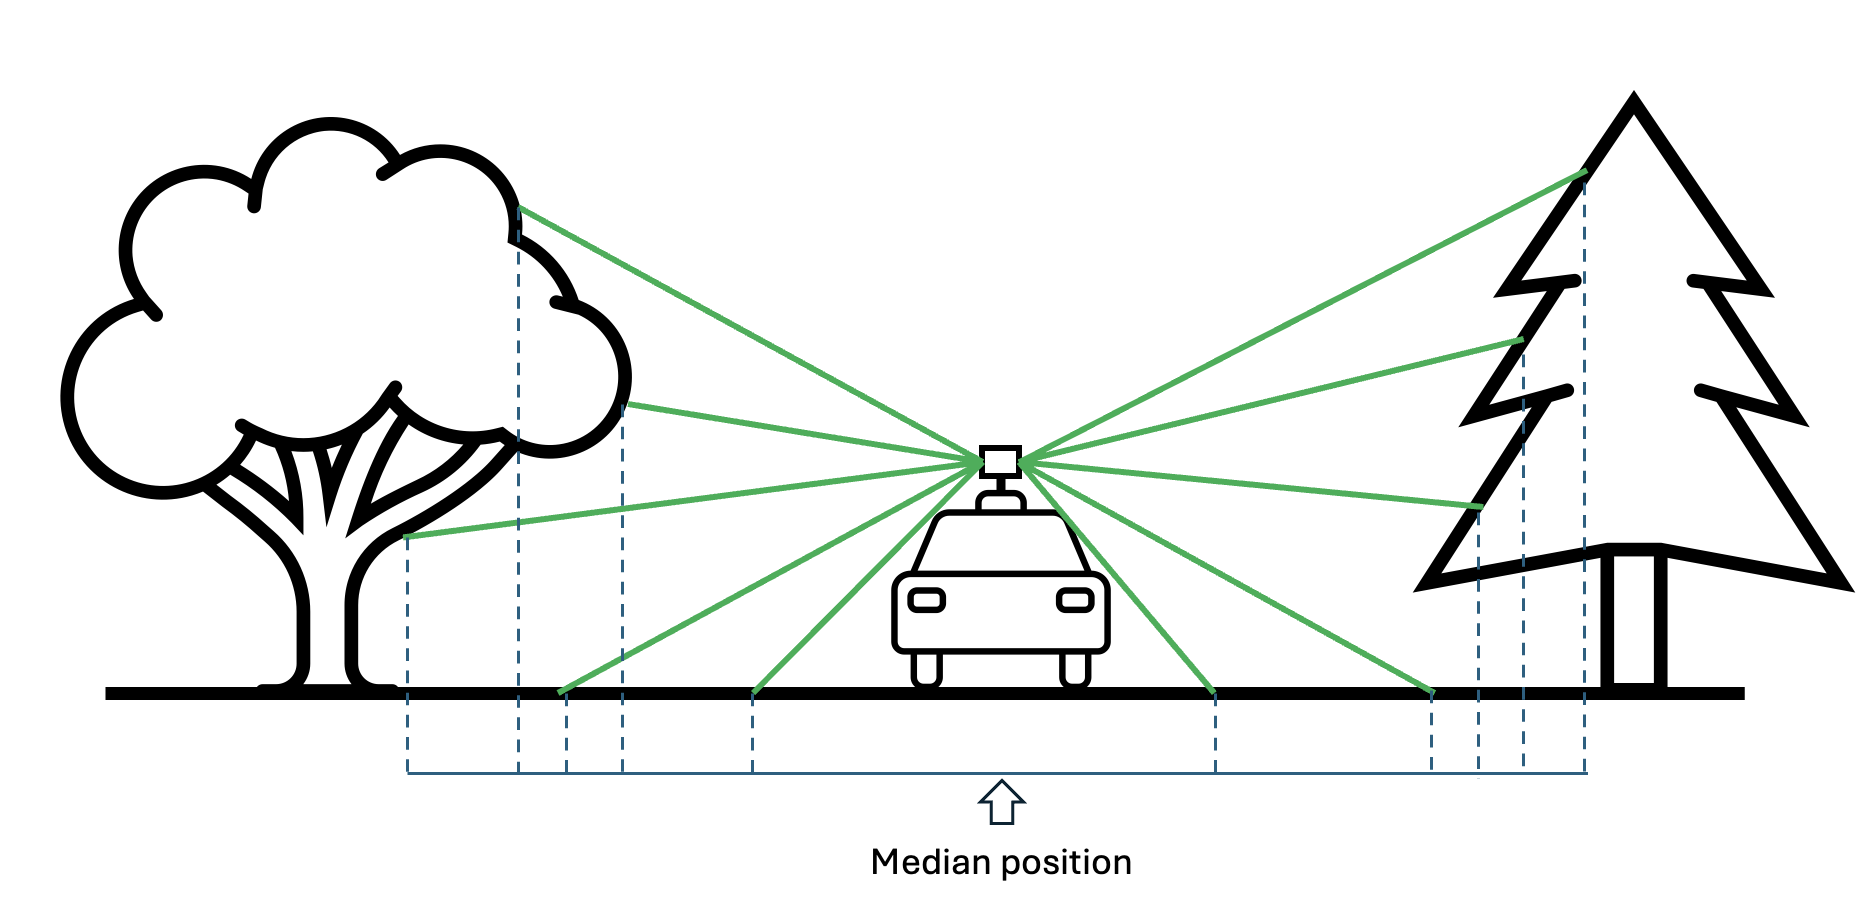
\includegraphics[width=\textwidth]{images/car_trace/window_median_illutstration}
    \caption{Visualization of the ideal situation.}
  \end{subfigure}
  \hfill
  \begin{subfigure}[b]{0.48\textwidth}
    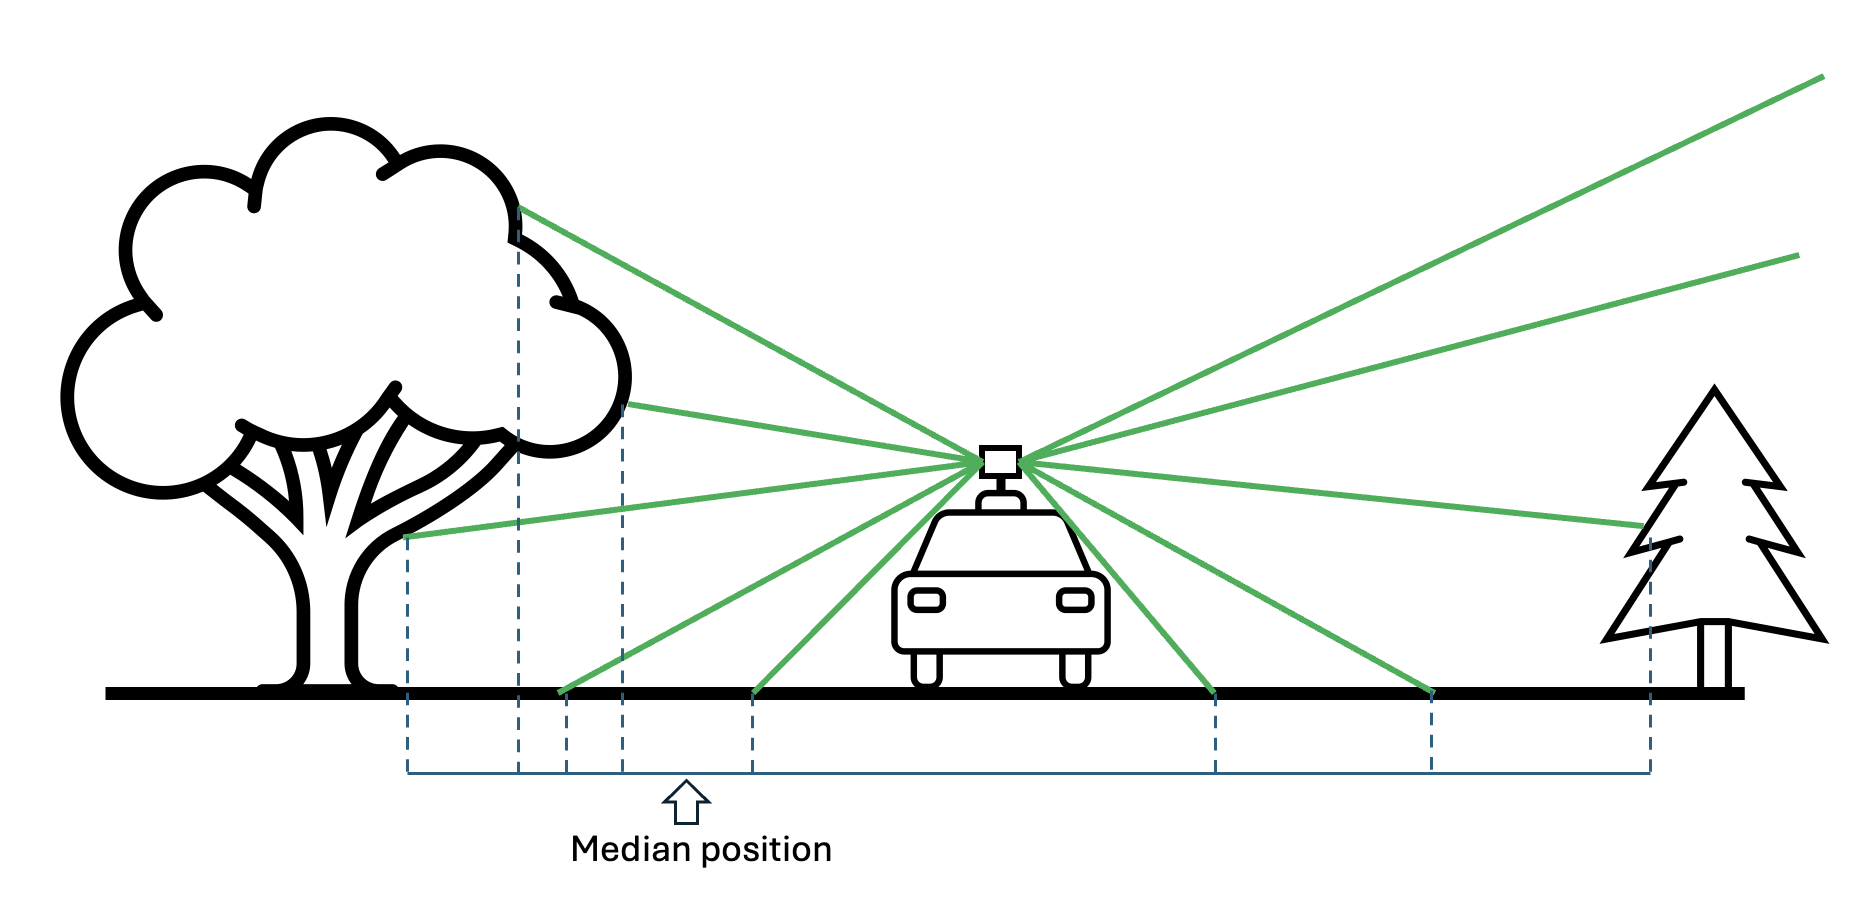
\includegraphics[width=\textwidth]{images/car_trace/window_median_illutstration_real}
    \caption{Uneven number of reflections.}
  \end{subfigure}
  \caption{Illustration of the Window Median algorithm, and it's defect: (a)~In the ideal situation both sides have the same amount of reflected points (b)~in typical scenarios, one side has more reflection.}
  \label{fig:window_median_illustration}
\end{figure}

The algorithm proceeds as follows:
\begin{enumerate}
  \item Select a temporal window of scanned points at regular time intervals.
  \item Compute the median of the $xy$-coordinates of all points within the window as the estimated vehicle position.
  \item Append the estimated positions sequentially to form a LineString geometry.
  \item Export the result to a GeoPackage file for subsequent evaluation.
\end{enumerate}

Despite its simplicity, this baseline method provides a surprisingly accurate approximation in the majority of cases. However, as shown in Figure~\ref{fig:window_median_result}, the estimate exhibits a systematic lateral bias: trees on the right side of the vehicle reflect more laser beams than the open left side, pulling the median toward the right.

\begin{figure}[htbp]
  \centering
  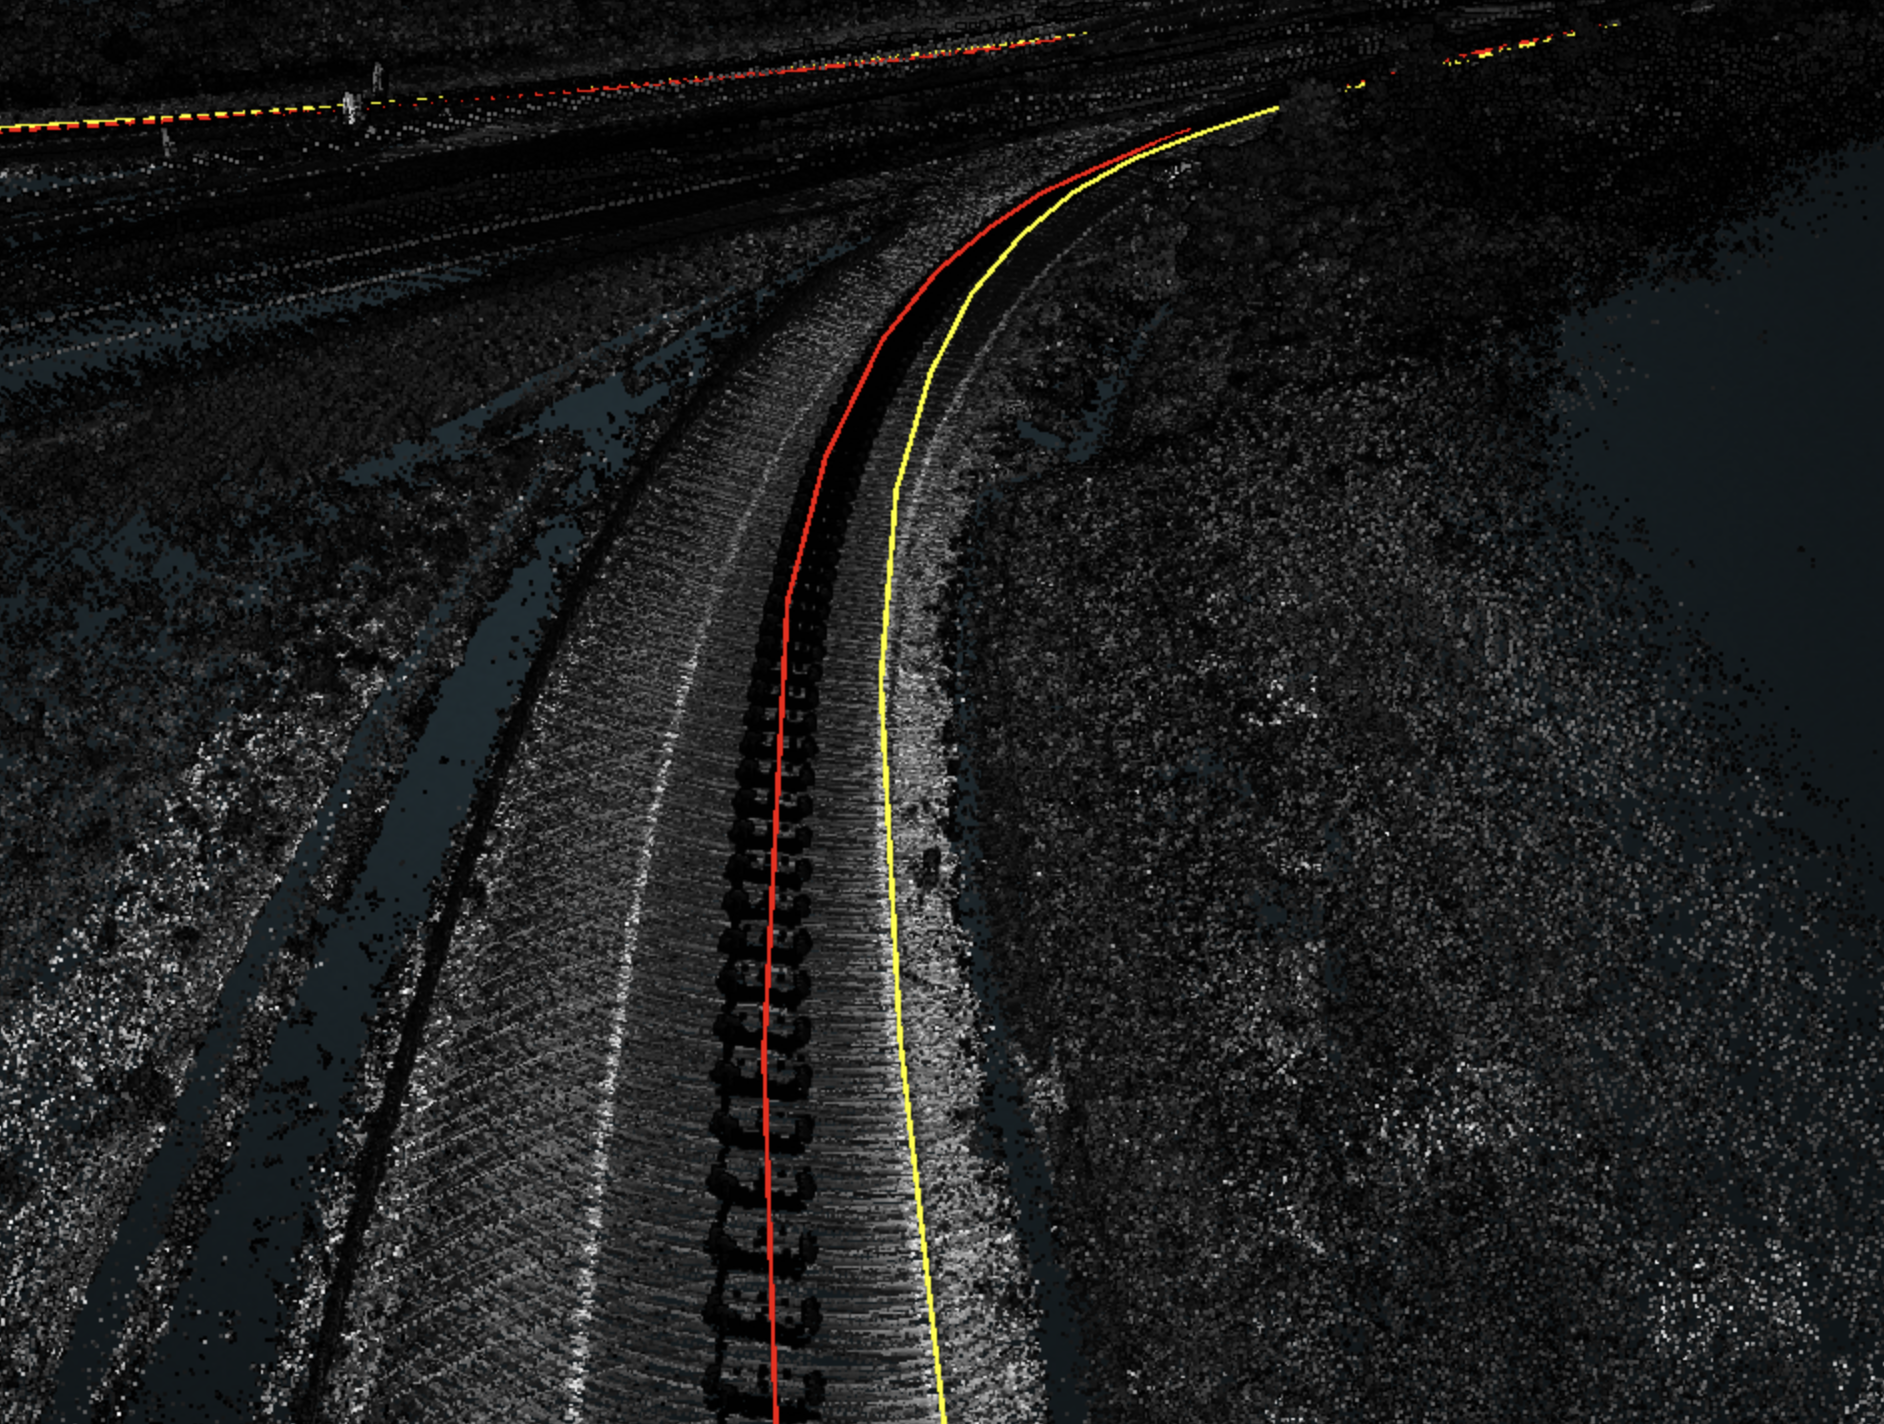
\includegraphics[width=0.7\textwidth]{images/car_trace/window_median_result}
  \caption{Comparison of the ground truth trajectory (red) and the Window Median baseline estimate (yellow). The systematic rightward bias is caused by asymmetric reflections from roadside vegetation.}
  \label{fig:window_median_result}
\end{figure}

\FloatBarrier
\subsection{Window Median with Ground Filtering}
\label{sec:window_median_v2}

This algorithm addresses the primary weakness of the baseline method. The key insight is that if points above a certain height threshold could be identified and excluded---particularly those reflected from elevated objects that are not symmetrically distributed---the resulting median would be significantly less biased. This approach assumes that downward-directed laser beams consistently produce valid ground returns.

The algorithm operates as follows:
\begin{enumerate}
  \item At regular time intervals, select a temporal window of points.
  \item Compute the median of the $xy$-coordinates as an initial position estimate.
  \item At the estimated position, determine the ground plane using iterative RANSAC-based plane fitting.
  \item Discard all points whose elevation exceeds the ground level by more than a specified offset $\Delta z$.
  \item Recompute the median of the remaining points as the refined vehicle position estimate.
\end{enumerate}

\begin{figure}[htbp]
  \centering
  \begin{subfigure}[b]{0.7\textwidth}
    \centering
    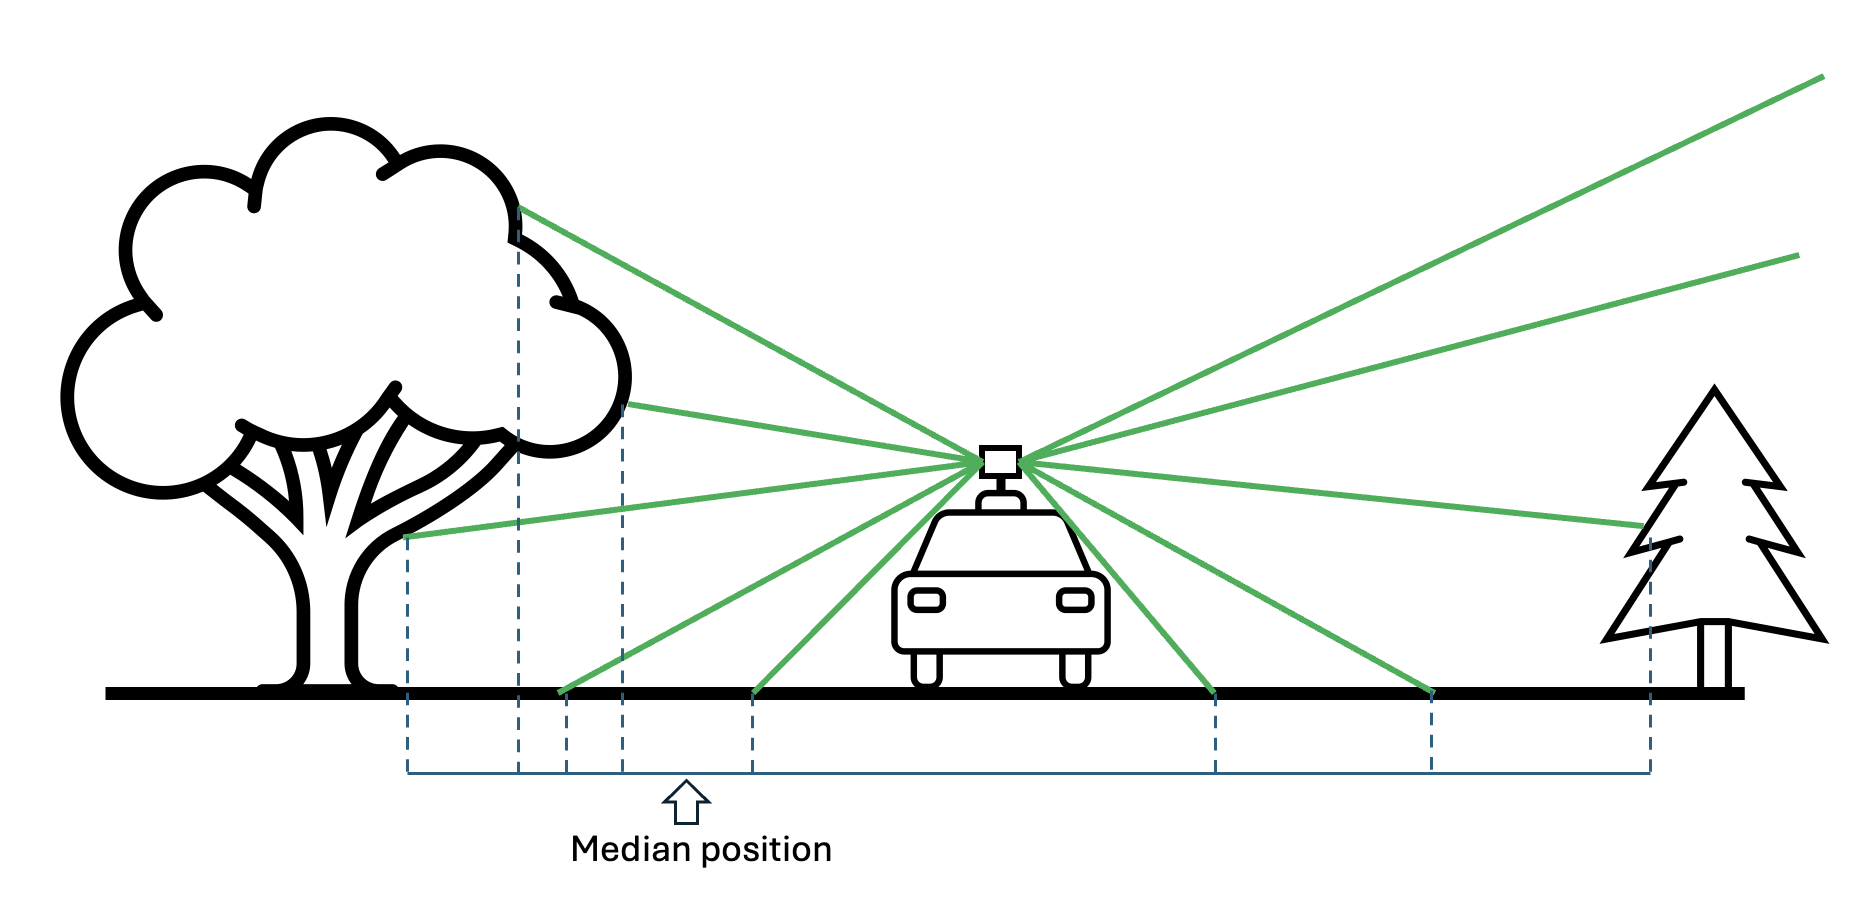
\includegraphics[width=\textwidth]{images/car_trace/window_median_illutstration_real}
    \caption{Biased baseline estimate.}
    \label{fig:wm_v2_bias}
  \end{subfigure}
  \\[0.5em]
  \begin{subfigure}[b]{0.7\textwidth}
    \centering
    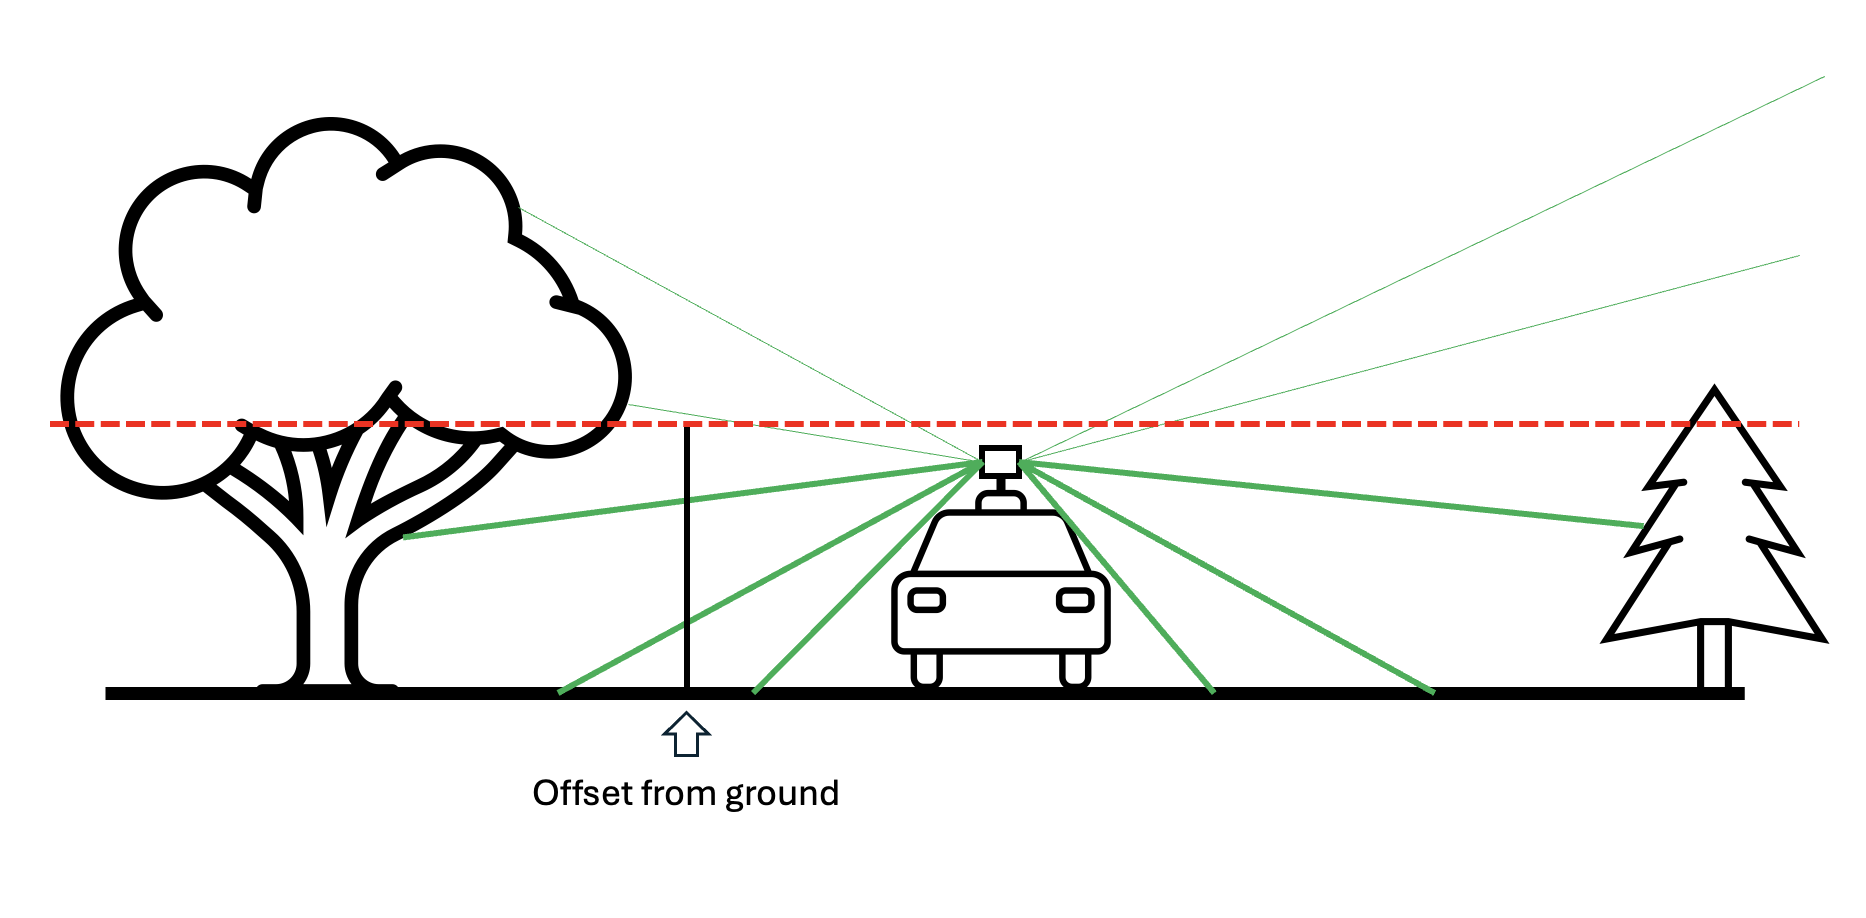
\includegraphics[width=\textwidth]{images/car_trace/window_median_v2_offset}
    \caption{Points above ground $+ \Delta z$ are discarded.}
    \label{fig:wm_v2_offset}
  \end{subfigure}
  \\[0.5em]
  \begin{subfigure}[b]{0.7\textwidth}
    \centering
    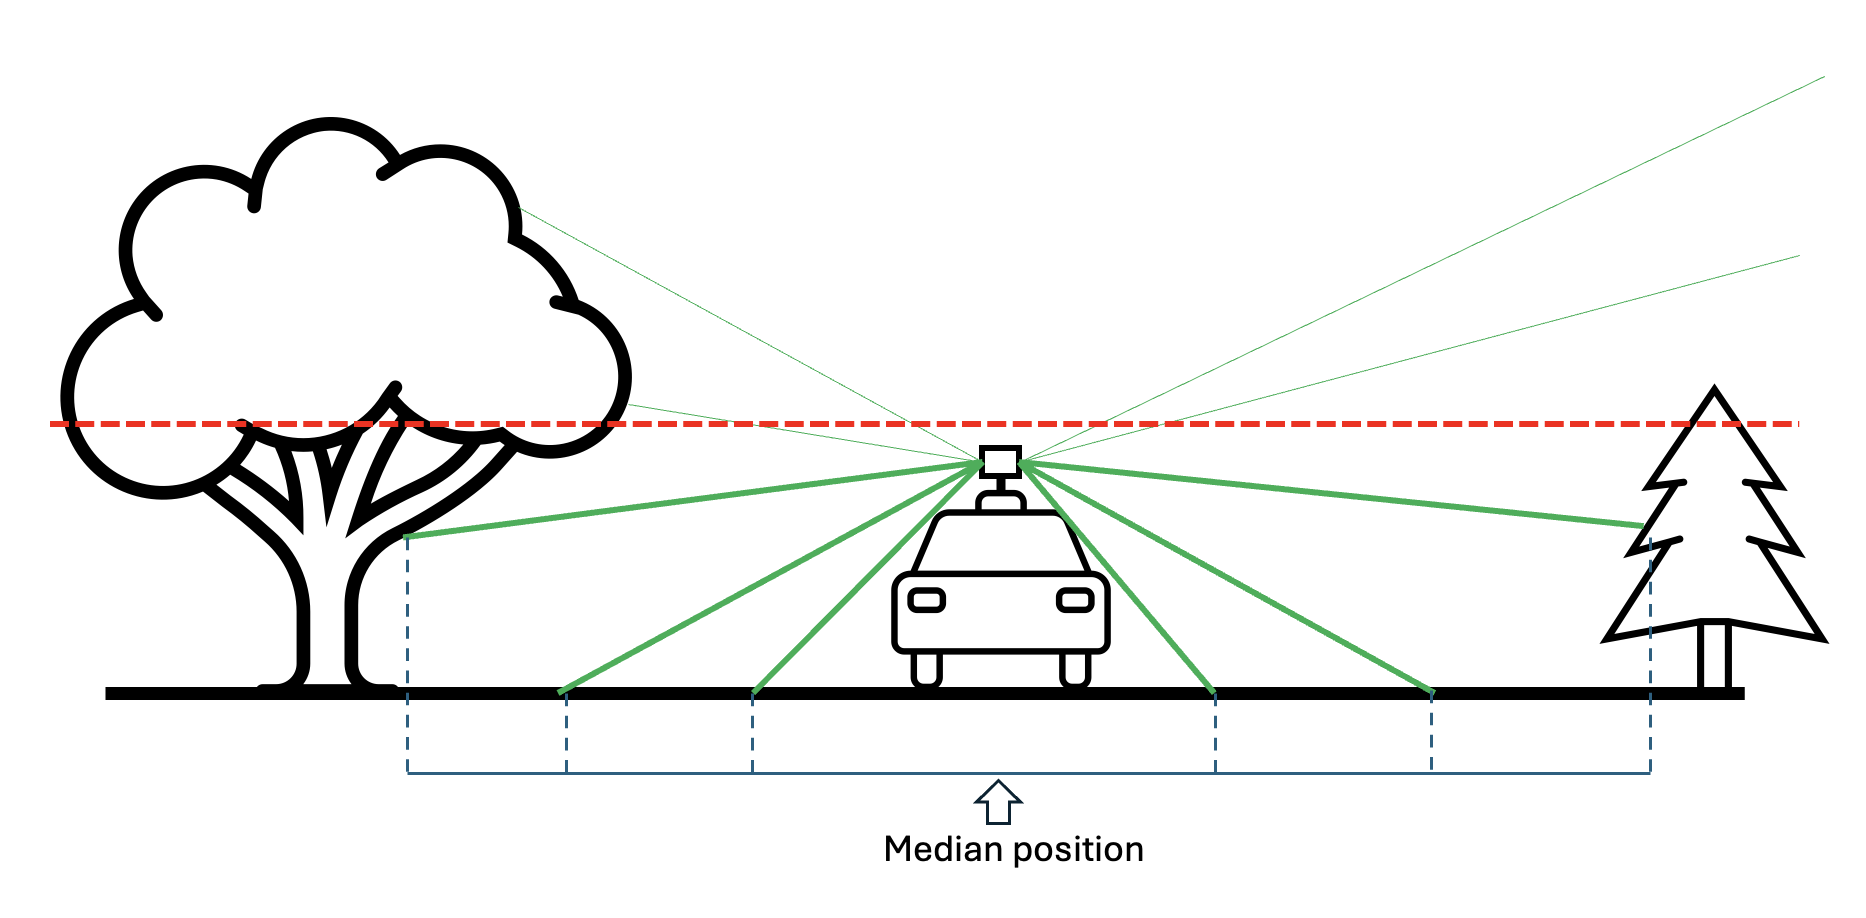
\includegraphics[width=\textwidth]{images/car_trace/window_median_v2}
    \caption{Corrected position estimate.}
    \label{fig:wm_v2_corrected}
  \end{subfigure}
  \caption{Illustration of the Window Median with Ground Filtering algorithm: (a)~the baseline produces a biased estimate; (b)~points above the ground plane plus an offset are removed; (c)~the recomputed median yields an improved estimate.}
  \label{fig:window_median_v2_illustration}
\end{figure}

As demonstrated in Figure~\ref{fig:window_median_v2_result}, this method provides a substantial improvement over the baseline. However, it is only effective when the initial (unfiltered) median estimate is already reasonably close to the true vehicle position.

\begin{figure}[htbp]
  \centering
  \includegraphics[width=0.7\textwidth]{images/car_trace/window_median_v2_result}
  \caption{Comparison of trajectory estimates: ground truth (red), Window Median baseline (yellow), and Window Median with Ground Filtering (orange).}
  \label{fig:window_median_v2_result}
\end{figure}

\FloatBarrier
\subsection{Pulse Line Intersection}
\label{sec:pulse_lines}

This algorithm exploits a geometric property of the LiDAR sensor's packet structure. As established in Section~\ref{sec:sensor}, points sharing the same GPS timestamp occupy an approximately $8^{\circ}$ unbounded angular sector originating from the LiDAR sensor. The center of this sector---the point from which the laser beams emanate---corresponds to the sensor position.

The algorithm is as follows:
\begin{enumerate}
  \item At regular intervals, select a packet (i.e., a set of points sharing a common GPS timestamp).
  \item Fit a regression line to the $xy$-coordinates of the packet's points using ordinary least squares.
  \item Advance through subsequent packets until a packet is found whose regression line forms a sufficiently large angle with the first.
  \item Compute the intersection of the two regression lines; this intersection is taken as the estimated sensor position.
\end{enumerate}

\noindent The geometric principle is illustrated in Figure~\ref{fig:pulse_lines}: since each packet's points lie along a narrow angular sector, their regression lines converge at the sensor location.

\begin{figure}[htbp]
  \centering
  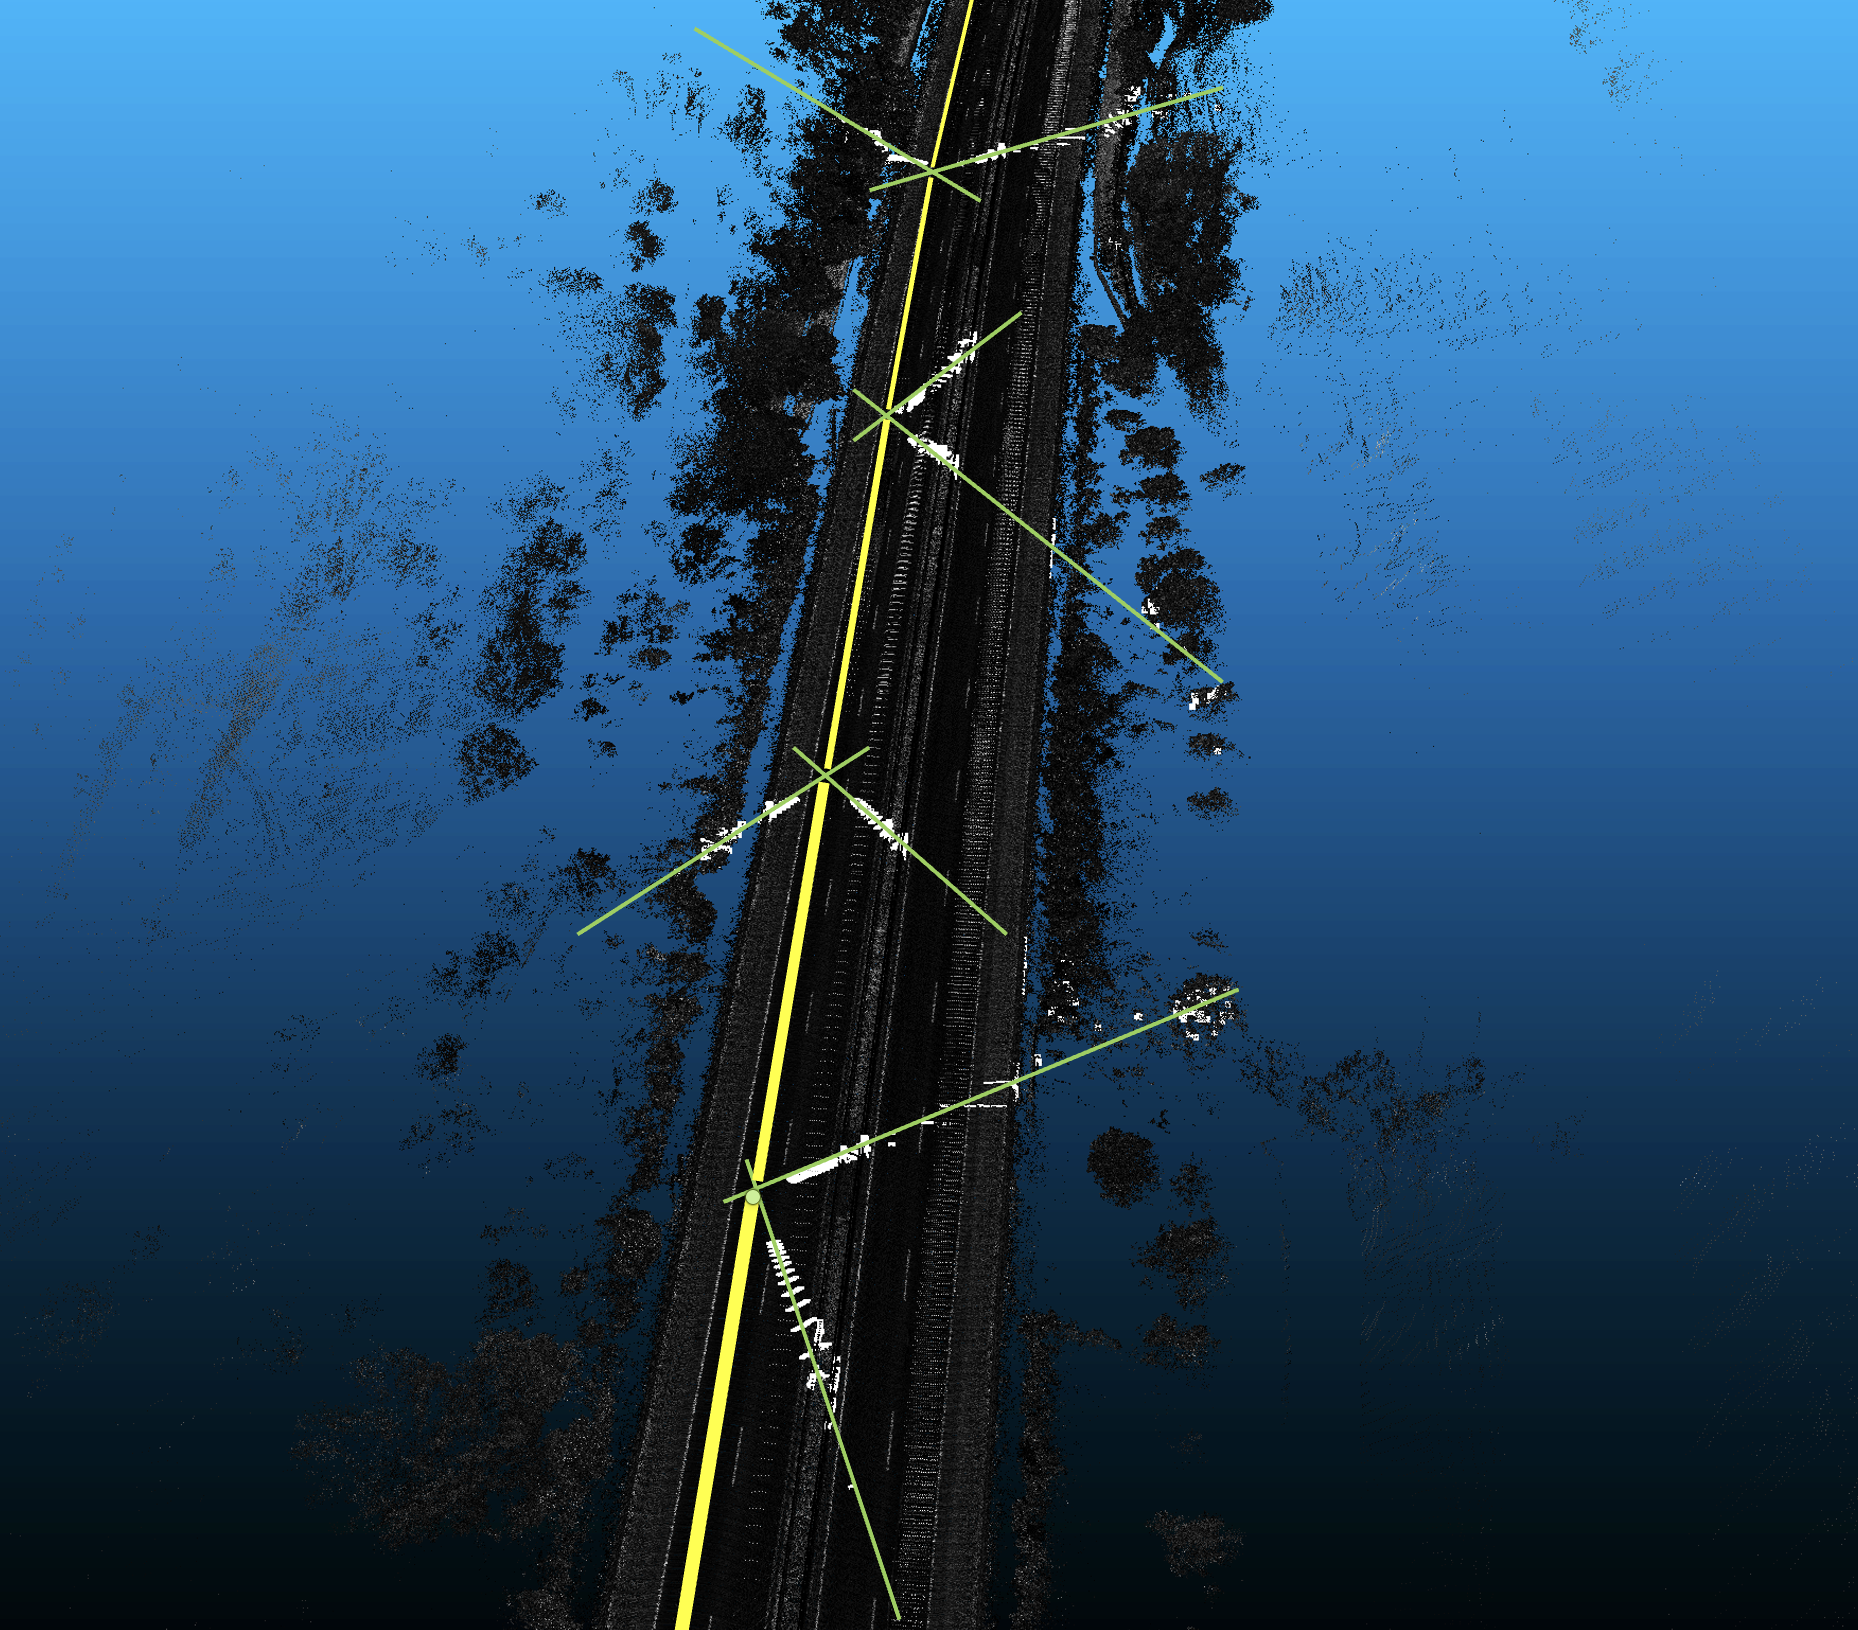
\includegraphics[width=0.7\textwidth]{images/car_trace/pulse_lines}
  \caption{The Pulse Line Intersection algorithm: regression lines fitted to individual packets intersect at the estimated sensor position.}
  \label{fig:pulse_lines}
\end{figure}

This algorithm produced highly accurate position estimates among all four methods (quantitative evaluation in Chapter~\ref{ch:eval}) and is therefore used as the default trajectory reconstruction method in the pipeline.

\FloatBarrier
\subsection{Closest Point Convergence}
\label{sec:closest_point}

This algorithm is based on the following observation: if the vehicle position is initialized at an arbitrary point and, for each successive packet, the estimate is updated to the point within that packet closest to the previous estimate, then the sequence of estimates converges to the point nearest to the LiDAR sensor.

The algorithm proceeds as follows:
\begin{enumerate}
  \item Initialize the estimated position at an arbitrary point.
  \item At regular time intervals, select a packet.
  \item Update the estimate to the point within the current packet that is closest (in the $xy$-plane) to the previous estimate.
  \item Repeat until all packets have been processed.
\end{enumerate}

\begin{figure}[htbp]
  \centering
  \begin{subfigure}[b]{0.48\textwidth}
    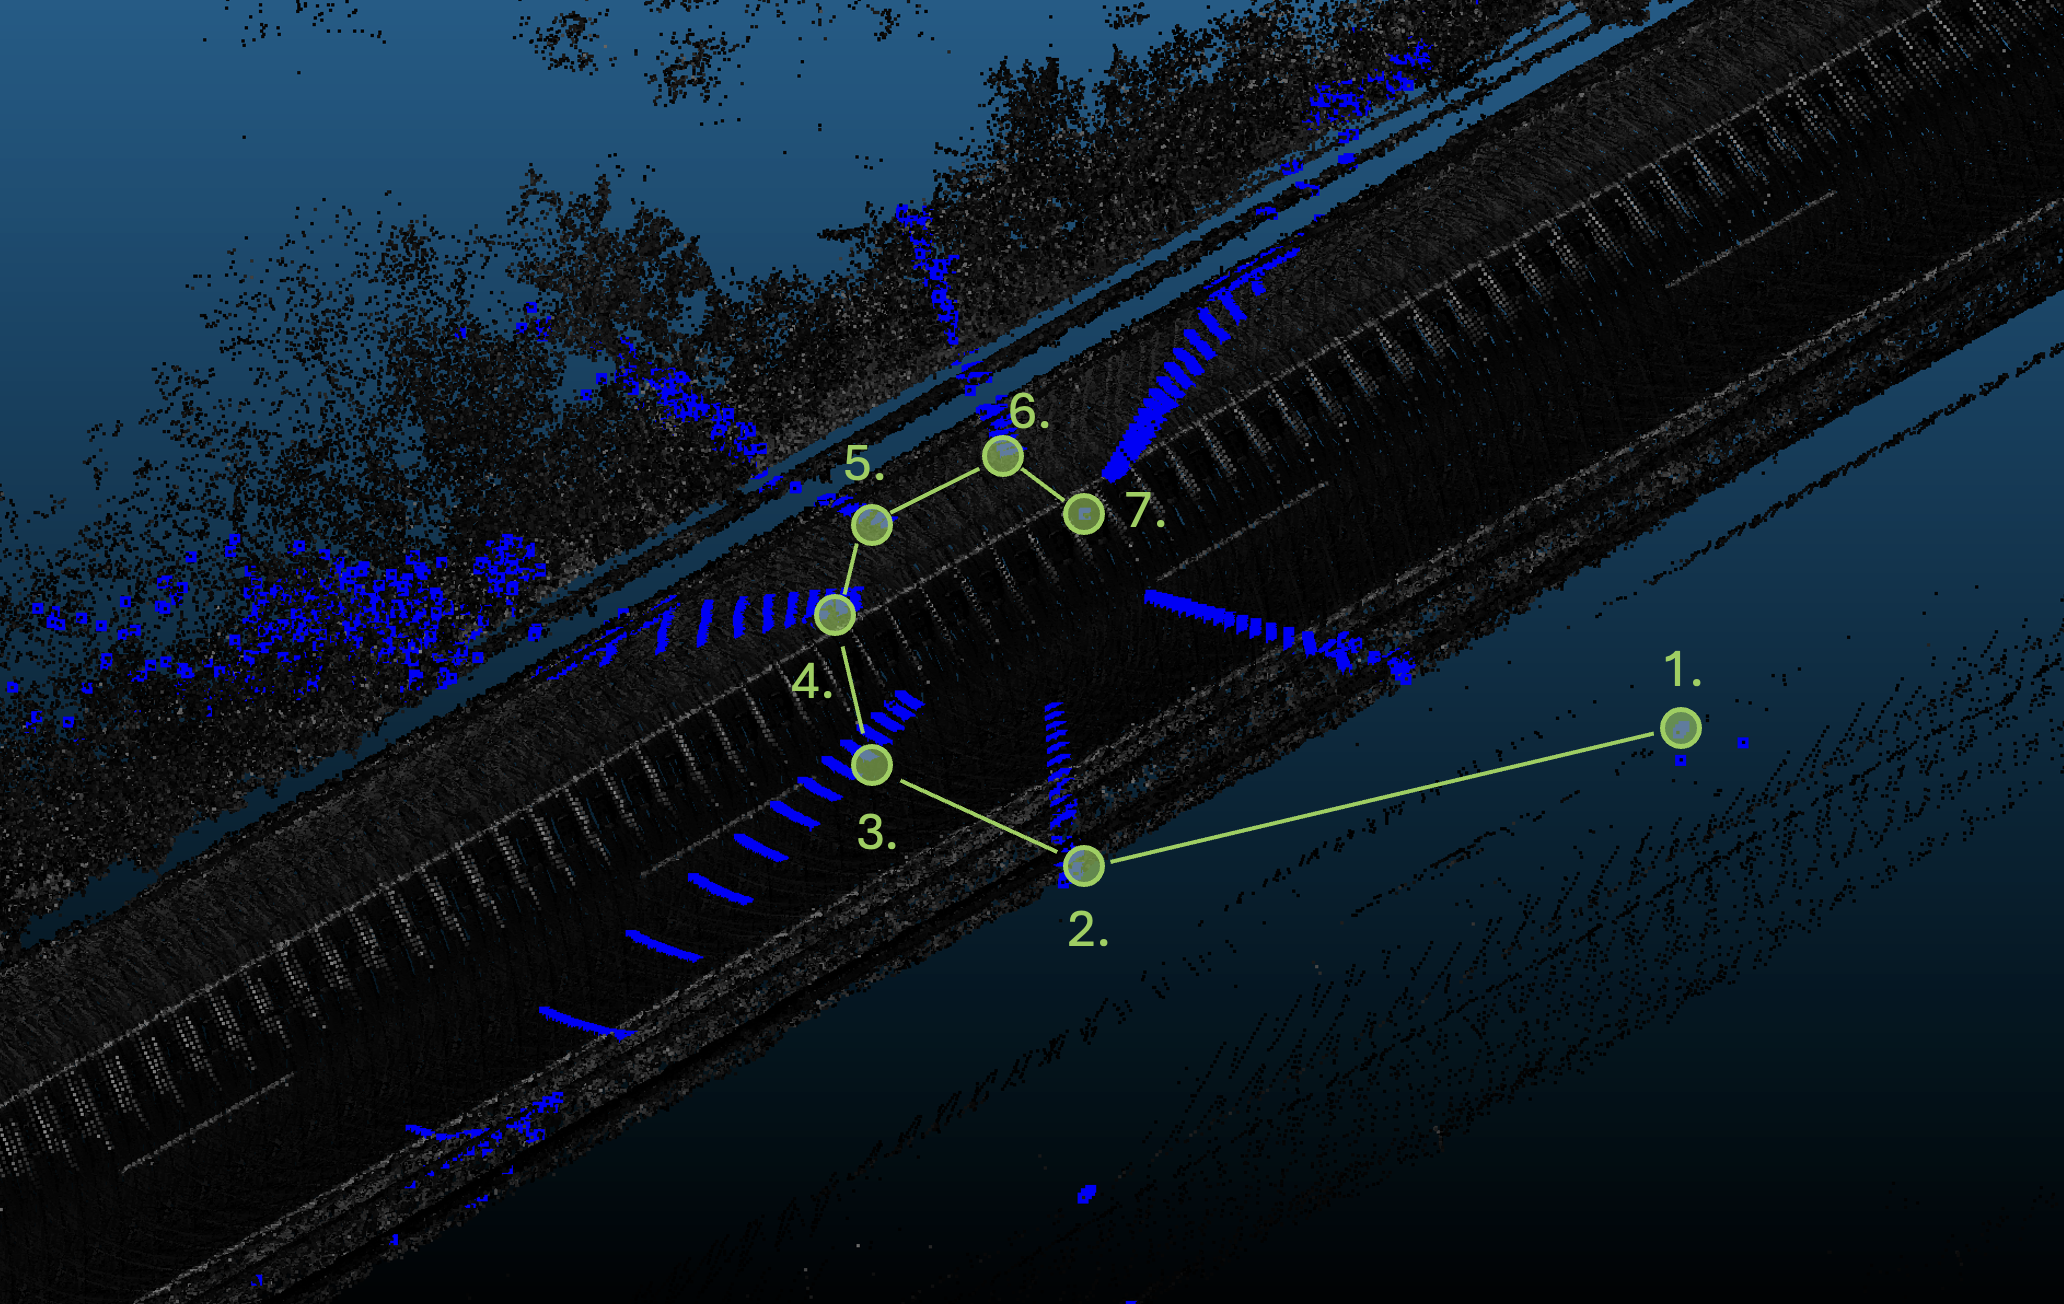
\includegraphics[width=\textwidth]{images/car_trace/closest_point_vis}
    \caption{Visualization of the iterative convergence process.}
    \label{fig:closest_point_vis}
  \end{subfigure}
  \hfill
  \begin{subfigure}[b]{0.48\textwidth}
    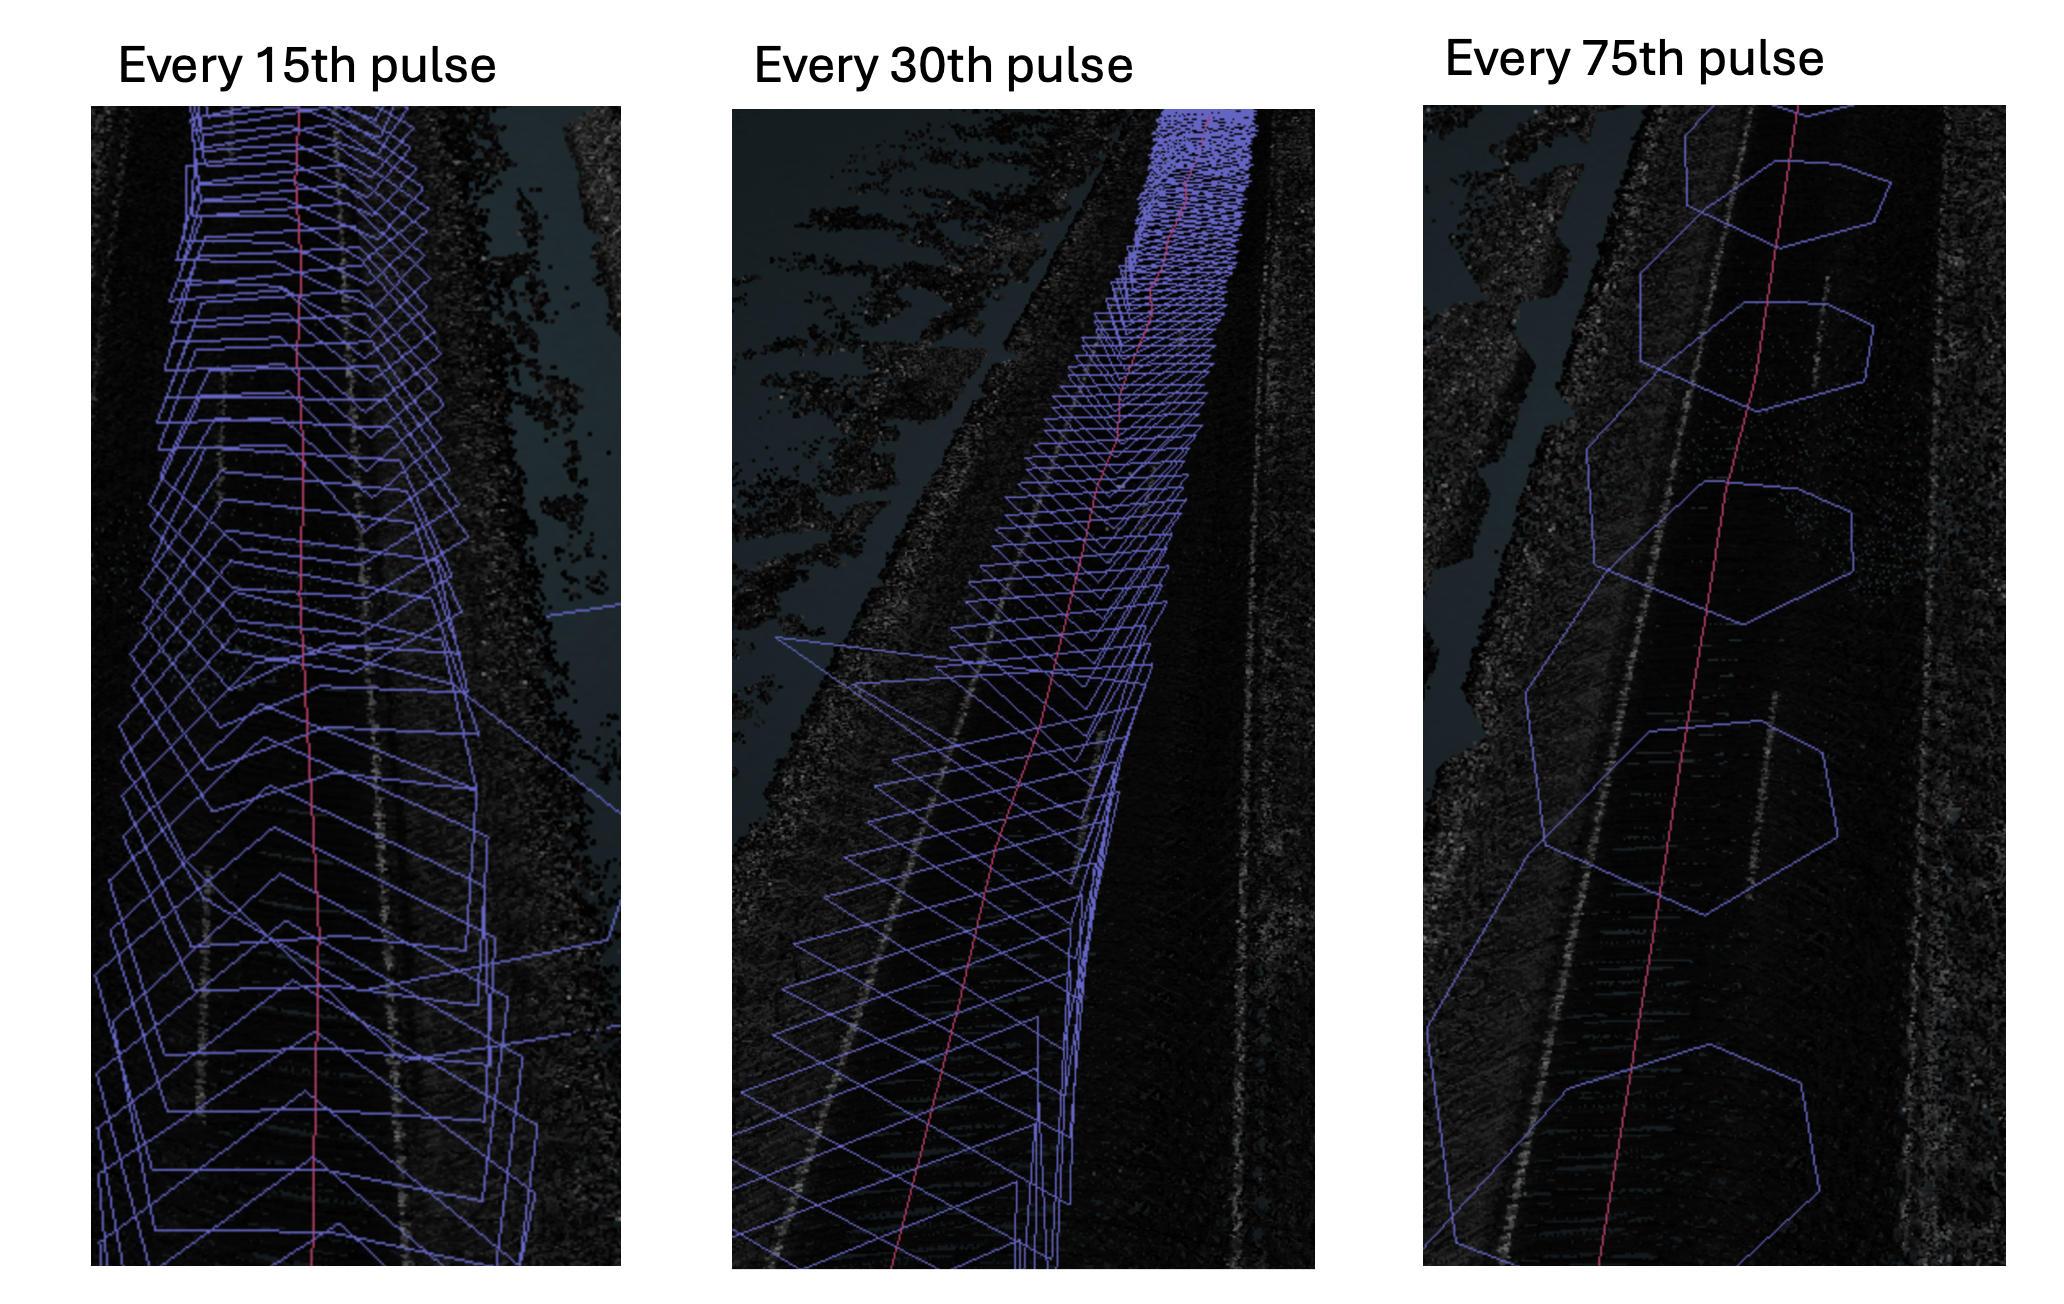
\includegraphics[width=\textwidth]{images/car_trace/closest_point_results}
    \caption{Output trajectory produced by the algorithm.}
    \label{fig:closest_point_results}
  \end{subfigure}
  \caption{The Closest Point Convergence algorithm: (a)~the iterative process by which successive estimates converge toward the sensor position; (b)~the resulting trajectory output.}
  \label{fig:closest_point}
\end{figure}

The output confirms that the convergence observation holds in practice. After applying a moving-window average followed by Gaussian smoothing, the resulting trajectory provides a usable estimate for subsequent pipeline stages.

\FloatBarrier
\subsection{Summary of Trajectory Reconstruction}
\label{sec:trace_summary}

Four trajectory reconstruction algorithms were presented, each providing adequate estimates under appropriate conditions. Table~\ref{tab:trace_algorithms} summarizes their characteristics. The pipeline uses the Pulse Line Intersection algorithm by default, as it consistently produced the most accurate estimates.

\begin{table}[htbp]
  \centering
  \caption{Summary of vehicle trajectory reconstruction algorithms.}
  \label{tab:trace_algorithms}
  \small
  \begin{tabular}{@{}lp{0.3\textwidth}p{0.35\textwidth}@{}}
    \hline
    Algorithm & Principle & Limitation \\
    \hline
    Window Median & Median of temporal window & Asymmetric reflection bias \\
    Window Median + GF & Ground-filtered median & Requires reasonable initial estimate \\
    Pulse Line Intersection & Regression line intersection & Requires sufficient angular separation \\
    Closest Point Convergence & Iterative nearest-point update & Requires post-processing (smoothing) \\
    \hline
  \end{tabular}
\end{table}

\FloatBarrier
%------------------------------------------------------------------
\section{Point Cloud Processing}
\label{sec:pointcloud_processing}

% TODO: This section will detail the following processing stages:
% - Binning along the vehicle trace
% - Distance-based clipping
% - RANSAC-based ground segmentation
% - Region-growing road surface detection
% - Intensity thresholding for road marking segmentation

\FloatBarrier
%------------------------------------------------------------------
\section{Line Fitting}
\label{sec:line_fitting}

% TODO: This section will detail the following stages:
% - Line extension RANSAC
% - Moving least squares refinement
% - Line labeling (solid vs. dashed)
